%  LaTeX support: latex@mdpi.com 
%  For support, please attach all files needed for compiling as well as the log file, and specify your operating system, LaTeX version, and LaTeX editor.

%=================================================================
\documentclass[notspecified,article,submit,moreauthors]{Definitions/mdpi}
%\documentclass[preprints,article,submit,moreauthors]{Definitions/mdpi}
% For posting an early version of this manuscript as a preprint, you may use "preprints" as the journal. Changing "submit" to "accept" before posting will remove line numbers.

%--------------------
% Class Options:
%--------------------
%----------
% journal
%----------
% Choose between the following MDPI journals:
% accountaudit, acoustics, actuators, addictions, adhesives, adolescents, aerobiology, aerospace, agriculture, agriengineering, agrochemicals, agronomy, ai, aichem, aieng, aimater, aimed, aipa, air, aisens, algorithms, allergies, alloys, amh, analog, analytica, analytics, anatomia, anesthres, animals, antibiotics, antibodies, antioxidants, applbiosci, appliedchem, appliedmath, appliedphys, applmech, applmicrobiol, applnano, applsci, aquacj, architecture, arm, arthropoda, asc, asi, astronautics, astronomy, atmosphere, atoms, audiolres, automation, axioms, bacteria, batteries, bdcc, beverages, biochem, bioengineering, biologics, biology, biomass, biomechanics, biomed, biomedicines, biomedinformatics, biomimetics, biomolecules, biophysica, bioresourbioprod, biosensors, biosphere, biotech, birds, blockchains, bloods, blsf, brainsci, breath, buildings, cancers, carbon, cardio, cardiogenetics, cardiovascmed, catalysts, cells, ceramics, challenges, chemengineering, chemistry, chemosensors, chemproc, children, chips, cimb, civileng, cleantechnol, climate, clinbioenerg, clinpract, clockssleep, cmd, cmtr, coasts, coatings, colloids, colorants, commodities, complexities, complications, compounds, computation, computers, condensedmatter, conservation, constrmater, cosmetics, covid, crops, cryo, cryptography, crystals, csmf, ctn, culture, curroncol, cyber, dairy, data, ddc, dentistry, dermato, dermatopathology, designs, devices, dhi, diabetology, diagnostics, dietetics, digital, disabilities, diseases, diversity, dna, drones, dynamics, earth, ebj, ecm, ecologies, edm, eesp, electricity, electrochem, electronicmat, electronics, encyclopedia, endocrines, energies, eng, engproc, entomology, entropy, environments, environremediat, epidemiologia, epigenomes, esa, est, fermentation, fibers, fintech, fire, fishes, fluids, foods, forecasting, forensicsci, forests, fossstud, foundations, fractalfract, fuels, future, futureinternet, futurepharmacol, futurephys, futuretransp, galaxies, gases, gastroent, gastrointestdisord, gastronomy, gels, genes, geographies, geohazards, geomatics, geometry, geosciences, geotechnics, geriatrics, germs, glacies, grasses, green, greenhealth, gucdd, hardware, hazardousmatters, healthcare, hearts, hemato, hematolrep, hep, heritage, higheredu, highthroughput, horticulturae, hospitals, hydrobiology, hydrogen, hydrology, hydropower, hygiene, idr, iic, ijem, ijerph, ijgi, ijmd, ijms, ijns, ijom, ijpb, ijt, ijtm, ijtpp, ime, immuno, informatics, information, infrastructures, inorganics, insects, instruments, inventions, iot, j, jaestheticmed, jal, jcdd, jcm, jcp, jcrm, jcs, jcto, jdad, jdb, jdream, jemr, jeta, jfb, jfmk, jgbg, jgg, jimaging, jlpea, jmahp, jmmp, jmms, jmp, jmse, jne, jnt, jof, joi, joitmc, joma, jop, joptm, jor, jox, jpbi, jytomed, jpm, jsan, jtaer, jvd, jzbg, kidneydial, kinasesphosphatases, knowledge, labmed, laboratories, lae, land, life, lights, limnolrev, lipidology, liquids, livers, logics, logistics, lubricants, lymphatics, machines, macromol, magnetism, magnetochemistry, make, marinedrugs, materials, materproc, mathematics, mca, measurements, medicina, medicines, medsci, membranes, merits, metabolites, metals, meteorology, methane, metrics, metrology, micro, microarrays, microbiolres, microelectronics, micromachines, microorganisms, microplastics, microwave, minerals, mining, mmphys, modelling, molbank, molecules, mps, msf, mti, multimedia, muscles, nanoenergyadv, nanomanufacturing, nanomaterials, ncrna, ndt, network, neuroglia, neuroimaging, neurolint, neurosci, nitrogen, notspecified, nursrep, nutraceuticals, nutrients, obesities, occuphealth, oceans, ohbm, onco, optics, oral, organics, organoids, osteology, oxygen, pandemics, parasites, parasitologia, particles, pathogens, pathophysiology, pediatrrep, pets, pharmaceuticals, pharmaceutics, pharmacoepidemiology, pharmacy, philosophies, photochem, photonics, phycology, physchem, physics, physiologia, plants, plasma, platforms, pollutants, polymers, polysaccharides, populations, poultry, powders, precipitation, precisoncol, preprints, proceedings, processes, prosthesis, proteomes, psf, psychiatryint, psychoactives, purification, quantumrep, quaternary, qubs, radiation, rdt, reactions, realestate, receptors, recycling, regeneration, remotesensing, reports, reprodmed, resources, rheumato, rjpm, robotics, rsee, ruminants, safety, sci, scipharm, sclerosis, seeds, sensors, separations, sexes, shi, signals, sinusitis, siuj, skins, smartcities, sna, societies, software, soilsystems, solar, solids, spectroscj, sports, standards, stats, std, stratsediment, stresses, surfaces, surgeries, suschem, sustainability, symmetry, synbio, systems, tae, targets, taxonomy, technologies, telecom, test, textiles, thalassrep, therapeutics, thermo, timespace, tomography, toxics, toxins, tph, transplantology, transportation, traumacare, traumas, tri, tropicalmed, universe, urbansci, uro, vaccines, vehicles, venereology, vetsci, vibration, virtualworlds, viruses, vision, waste, water, welding, wem, wevj, wild, wind, women, world, zoonoticdis

%---------
% article
%---------
% The default type of manuscript is "article", but can be replaced by: 
% abstract, addendum, article, benchmark, book, bookreview, briefcommunication, briefreport, casereport, changes, clinicopathologicalchallenge, comment, commentary, communication, conceptpaper, conferenceproceedings, correction, conferencereport, creative, datadescriptor, discussion, entry, expressionofconcern, extendedabstract, editorial, essay, erratum, fieldguide, hypothesis, interestingimages, letter, meetingreport, monograph, newbookreceived, obituary, opinion, proceedingpaper, projectreport, reply, retraction, review, perspective, protocol, shortnote, studyprotocol, supfile, systematicreview, technicalnote, viewpoint, guidelines, registeredreport, tutorial,  giantsinurology, urologyaroundtheworld
% supfile = supplementary materials

%----------
% submit
%----------
% The class option "submit" will be changed to "accept" by the Editorial Office when the paper is accepted. This will only make changes to the frontpage (e.g., the logo of the journal will get visible), the headings, and the copyright information. Also, line numbering will be removed. Journal info and pagination for accepted papers will also be assigned by the Editorial Office.

%------------------
% moreauthors
%------------------
% If there is only one author the class option oneauthor should be used. Otherwise use the class option moreauthors.

%---------
% pdftex
%---------
% The option pdftex is for use with pdfLaTeX. Remove "pdftex" for (1) compiling with LaTeX & dvi2pdf (if eps figures are used) or for (2) compiling with XeLaTeX.

%=================================================================
% MDPI internal commands - do not modify
\firstpage{1} 
\makeatletter 
\setcounter{page}{\@firstpage} 
\makeatother
\pubvolume{1}
\issuenum{1}
\articlenumber{0}
\pubyear{2026}
\copyrightyear{2026}
%\externaleditor{Name Surname} % More than 1 editor, please add `` and '' before the last editor name
\datereceived{ } 
\daterevised{ } % Comment out if no revised date
\dateaccepted{ } 
\datepublished{ } 
%\datecorrected{} % For corrected papers: "Corrected: XXX" date in the original paper.
%\dateretracted{} % For retracted papers: "Retracted: XXX" date in the original paper.
%\doinum{} % Used for some special journals, like molbank
%\pdfoutput=1 % Uncommented for upload to arXiv.org
%\CorrStatement{yes}  % For updates
%\longauthorlist{yes} % For many authors that exceed the left citation part
%\IsAssociation{yes} % For association journals
\setlength{\headheight}{20pt}

%=================================================================
% Add packages and commands here. The following packages are loaded in our class file: fontenc, inputenc, calc, indentfirst, fancyhdr, graphicx, epstopdf, lastpage, ifthen, float, amsmath, amssymb, lineno, setspace, enumitem, mathpazo, booktabs, titlesec, etoolbox, tabto, xcolor, colortbl, soul, multirow, microtype, tikz, totcount, changepage, attrib, upgreek, array, tabularx, pbox, ragged2e, tocloft, marginnote, marginfix, enotez, amsthm, natbib, hyperref, cleveref, scrextend, url, geometry, newfloat, caption, draftwatermark, seqsplit
% cleveref: load \crefname definitions after \begin{document}
\graphicspath{{figures/}}

%=================================================================
% Please use the following mathematics environments: Theorem, Lemma, Corollary, Proposition, Characterization, Property, Problem, Example, ExamplesandDefinitions, Hypothesis, Remark, Definition, Notation, Assumption
% For proofs, please use the proof environment (the amsthm package is loaded by the MDPI class).

%=================================================================
% Full title of the paper (Capitalized)
\Title{Trust-Stream Evaluation of Trust-Guided Task Allocation in Low-Altitude UAV Networks}

% Author Orchid ID: enter ID or remove command
\newcommand{\orcidauthorA}{0000-0000-0000-000X} % Add \orcidA{} behind the author's name
%\newcommand{\orcidauthorB}{0000-0000-0000-000X} % Add \orcidB{} behind the author's name

% Authors, for the paper (add full first names)
\Author{Anonymous Authors}

%\longauthorlist{yes}

% MDPI internal command: Authors, for metadata in PDF
\AuthorNames{Anonymous Authors}

% Affiliations / Addresses (Add [1] after \address if there is only one affiliation.)
\address{%
Department of Computer Science and Engineering, Anonymous Institution}

% Contact information of the corresponding author
\corres{Correspondence: to be provided after peer-review anonymization is removed.}

% Current address and/or shared authorship
%\firstnote{Current address: Affiliation.}  
% Current address should not be the same as any items in the Affiliation section.

%\secondnote{These authors contributed equally to this work.}
% The commands \thirdnote{} till \eighthnote{} are available for further notes.

%\simplesumm{} % Simple summary

%\conference{} % An extended version of a conference paper

% Abstract (Do not insert blank lines, i.e. \\) 
\abstract{Trust scores are useful in a cooperative UAV mission only when they inform an operational decision. This paper studies that link at the trust-stream level. We construct five normalized evidence streams---behavior, communication, energy, task execution, and history---and train a supervised multi-head network to estimate node risk and auxiliary task-allocation actions. The executable artifact is deliberately narrower than a full multi-agent reinforcement-learning system: it uses simulator labels during offline training, freezes the model for evaluation, and does not learn from environment rewards or deployment trajectories. On 50 held-out generated seeds with 15 UAVs and a 30\% malicious-node ratio, the model obtains 94.4\% accuracy and a 91.8\% F-score. A same-feature MLP obtains 94.7\% and 92.1\%, respectively; neither difference is statistically significant. A model-based task-allocation simulation yields a 90.5\% success proxy for the proposed configuration and 88.3\% for the MLP, but this comparison is descriptive because the simulator applies mechanism-specific allocation rules. On one short ns-3-derived trace, the proposed model achieves 80.0\% accuracy and 40.0\% recall, trailing three rule-based adapters in recall. The results therefore establish reproducibility and feasibility only within the generated trust-stream setting. Claims about online adaptation, packet-level robustness, communication cost, and flight deployment require independent experiments.}

% Keywords
\keyword{UAV networks; trust management; task allocation; zero trust; reproducible simulation}
  
% The fields PACS, MSC, and JEL may be left empty or commented out if not applicable
%\PACS{J0101}
%\MSC{}
%\JEL{}

%%%%%%%%%%%%%
% Only for the journal Diversity
%\LSID{\url{http://}}

%%%%%%%%%%%%%
% Only for the journal Applied Sciences
%\featuredapplication{Authors are encouraged to provide a concise description of the specific application or a potential application of the work. This section is not mandatory.}
%%%%%%%%%%%%%

%%%%%%%%%%%%%
% Only for the journal Data
%\dataset{DOI number or link to the deposited data set if the data set is published separately. If the data set shall be published as a supplement to this paper, this field will be filled by the journal editors. In this case, please submit the data set as a supplement.}
%\datasetlicense{License under which the data set is made available (CC0, CC-BY, CC-BY-SA, CC-BY-NC, etc.)}

%%%%%%%%%%%%%
% Only for the journal BioTech, Fishes, Neuroimaging and Toxins
%\keycontribution{The breakthroughs or highlights of the manuscript. Authors can write one or two sentences to describe the most important part of the paper.}

%%%%%%%%%%%%%
% Only for the journal Encyclopedia
%\encyclopediadef{For entry manuscripts only: please provide a brief overview of the entry title instead of an abstract.}

%%%%%%%%%%%%%
% Different journals have different requirements. Please check the specific journal guidelines in the "Instructions for Authors" on the journal's official website.
%\addhighlights{yes}
%\renewcommand{\addhighlights}{%%%%%%%%%%%%%%%%%%%%%%%%%%%%%%%%%%%%%%%%%%%%%%%%%%%%%%%%%%%%
%\noindent The goal is to increase the discoverability and readability of the article via search engines and other scholars. Highlights should not be a copy of the abstract, but a simple text allowing the reader to quickly and simplified find out what the article is about and what can be cited from it. Each of these parts should be devoted up to 2~bullet points.\vspace{3pt}\\
%\textbf{What are the main findings?}
% \begin{itemize}[labelsep=2.5mm,topsep=-3pt]
% \item First bullet.
% \item Second bullet.
% \end{itemize}\vspace{3pt}
%\textbf{What are the implications of the main findings?}
% \begin{itemize}[labelsep=2.5mm,topsep=-3pt]
% \item First bullet.
% \item Second bullet.
% \end{itemize}
%}

%%%%%%%%%%%%%
\begin{document}

%%%%%%%%%%%%%
\section{Introduction}
UAV swarms used for inspection, sensing, and emergency response rely on nodes that remain inside the mission after admission. A valid identity is therefore not sufficient evidence of trustworthy behavior. A compromised node can selectively forward traffic, falsify a task result, or alternate between benign and harmful behavior while retaining the privileges granted by its earlier history. Dynamic topology and intermittent links make those behaviors difficult to distinguish from ordinary failures \cite{kundu2024survey,noor2020fanet}.

Trust management addresses this problem by updating a node score from recent observations. Existing schemes use fuzzy fusion, anomaly profiles, provenance, or group decisions \cite{benfriha2024fuba,akram2024galtrust,ge2021uavpro,hu2025gdm}. Their scores, however, are often evaluated only as detector outputs. In a mission, the practical question is what changes after a node becomes risky: whether it may receive a sensitive task, how much traffic it may relay, and when it should be isolated. This study examines that narrower trust-to-allocation question.

We present MTIM as a reproducible proof of concept rather than a deployment-ready zero-trust architecture. The artifact generates five trust-factor streams, fits a supervised multi-head network, and uses its risk output in a model-based task-allocation simulation. Although the architecture was motivated by parameterized multi-agent decision making, the released training procedure is not reinforcement learning: there is no sampled return, Bellman target, policy-gradient update, or online interaction with an environment. Calling the executable model MARL would therefore overstate what was implemented.

The study asks two bounded questions. First, can temporal summaries of generated trust streams distinguish constant, dormant, and on--off attackers on held-out random seeds? Second, under the allocation rules encoded in the same simulator, does trust-guided selection improve a task-success proxy? The answer to the first question is positive within the generator but no better than a same-feature MLP. The second result is suggestive rather than causal because the task simulator contains mechanism-specific rules. A short ns-3-derived trace is included to expose, rather than hide, the remaining packet-level gap.

\textbf{Problem statement.}
This paper addresses a trust-layer decision problem for fixed identities: how should a risk estimate derived from noisy multi-factor evidence affect a subsequent task-allocation decision? The empirical scope is a generated trust-stream benchmark. It does not cover admission control, Sybil resistance, real-time distributed execution, or flight deployment.

Figure~\ref{fig:Proposed} gives the intended deployment architecture. Only its trust-stream classifier and allocation proxy are exercised in the released artifact. The contributions are consequently limited to the following:

\begin{itemize}
    \item a documented generator for behavioral, communication, energy, task, and historical trust streams under three temporal attack patterns;
    \item a reproducible supervised multi-head model and same-feature LR/MLP comparators evaluated on disjoint training and evaluation seeds; and
    \item an explicit negative result: the proposed risk head does not outperform the same-feature MLP, and the available packet-trace check is too small to establish external validity.
\end{itemize}

The remainder of this paper reviews related work, defines the intended architecture and executable subset, reports the trust-stream experiments and packet-trace check, and closes with limitations.

\section{Related Work}
Trust evaluation for UAV networks now includes reputation models, evidence fusion, blockchain support, and learning-based designs. Yet low-altitude UAV studies rarely integrate zero-trust verification, distributed trust learning, uncertainty aggregation, and mission incentives. We review three related areas: UAV trust management, zero-trust assessment, and MARL for UAV networking and security.

\subsection{Trust Management in UAV and FANET Systems}
Recent surveys show that trust management has become a core security primitive in FANETs, where dynamic topology, intermittent links, and resource limits make purely identity-based protection insufficient \cite{kundu2024survey,noor2020fanet,brik2020fluav,nguyen2021fliotsurvey,qu2021dflun}. Existing schemes fall into three categories: behavior-centric trust analytics, distributed or blockchain-supported trust, and learning-enhanced trust evaluation.

Behavior-centric trust evaluation widely uses fuzzy and evidence-fusion methods to combine heterogeneous observations. Benfriha et al. proposed FUBA, which uses fuzzy logic to integrate indicators such as RSSI, packet delivery ratio, delay, battery level, and humidity to identify insider threats in FANETs \cite{benfriha2024fuba}. Li et al. developed an adaptive multi-granularity trust management scheme for UAV visual sensor security under adversarial attacks, where coarse- and fine-grained evidence is fused to improve robustness against known and unknown threats \cite{li2025multigranularity}. Akram et al. introduced GALTrust, which combines generative adversarial learning with type-2 fuzzy logic to improve adaptability to emerging malicious behaviors in spatial crowdsourcing drone services \cite{akram2024galtrust}. More recent federated-security studies also move trust assessment toward collaborative anomaly detection, including FL-based intrusion detection for FANETs, multimodal swarm anomaly detection, and communication-efficient FL for resource-constrained UAV-IoT systems \cite{ceviz2025flids,lu2024swarmfl,gad2024somkd}. These studies significantly enrich trust evidence modeling. Their remaining limitation for the problem considered here is not that they cannot detect insider behavior at all, but that fuzzy, profile-based, or task-specific fusion can become sensitive to distribution shifts when the malicious population is dense and attack timing is deliberately evasive.

A second line of work improves trust persistence and auditability through distributed storage or hierarchical trust exchange. Ge et al. developed a provenance-aware distributed trust model for resilient UAV networks, highlighting the value of peer-to-peer evidence tracing in hostile environments \cite{ge2021uavpro}. Zuo et al. proposed a hierarchical blockchain-based trust measurement method for drone clusters to address trust inheritance, cross-cluster re-evaluation, and historical trust verification under dynamic node entry and exit \cite{zuo2023blockchain}. Akram et al. proposed TMIoDT, which integrates digital twins, blockchain, and deep-learning-based intrusion detection to secure Open RAN-based Internet of Drone Things applications \cite{akram2024tmiodt}. Closely related secure-FL frameworks have further explored malicious-node detection and trusted collaboration through blockchain-supported service provisioning, privacy-preserving IoDT security, and hierarchical federated aggregation \cite{abubaker2022blockchained,akram2023chained,zheng2024tinyfl,tong2024hierarchicalfl}. Related work on secure quantum federated learning in UAV-assisted wireless networks further indicates that trust-enhanced game incentives can improve participation quality and strengthen learning robustness under strategic behavior \cite{trustgame_qfl_uav}. More recently, Hu et al. proposed GDM-DTM for malicious-node detection in low-altitude UAV networks by combining group decision making with dynamic trust management \cite{hu2025gdm}. These schemes improve distributed credibility, trust persistence, and malicious-node detection. For our setting, the central gap is that the trust state is usually treated as an assessment output rather than as the basis for learned reward, penalty, and task-allocation decisions.

\subsection{Zero-Trust and Continuous Trust Assessment}
Zero trust shifts security from perimeter-based assumptions to continuous, resource-centric verification. The NIST zero-trust architecture defines this paradigm through the principle of ``never trust, always verify'' and replaces implicit perimeter-based trust with continuous, context-aware verification \cite{rose2020zero}. Building on this idea, Wang et al. proposed a zero-trust-driven collaborative intrusion detection framework for IoT that uses continuous trust assessment to support distributed security decisions \cite{wang2025continuous}. In the UAV and 6G context, Al Ridhawi and Aloqaily integrated zero trust, digital twins, federated learning, and blockchain into a UAV-enabled 6G framework, highlighting the broader relevance of decentralized trust enforcement in highly dynamic aerial networks \cite{ridhawi2023zerotrust6g}. In the UAV authentication domain, Wang et al. introduced a context-aware trust evaluation model for malicious UAV detection during authentication, showing that trust can also be injected into the authentication stage rather than being treated purely as a post hoc reputation signal \cite{wang2026wolf}.

Zero trust is particularly relevant to low-altitude UAV swarms: node roles may change during flight, links may appear and disappear rapidly, and local observations may be incomplete or noisy. Trust decisions cannot be based solely on prior membership or static credentials, but must be continuously updated from current observations, device status, communication behavior, and mission context. Therefore, trust decisions should be dynamic, uncertainty-aware, and resource-conscious rather than static or binary.

These studies move trust evaluation closer to continuous verification. Nevertheless, the current zero-trust literature still focuses mainly on authentication, access control, or intrusion detection. It does not fully address how trust should evolve online in low-altitude UAV swarms when heterogeneous evidence from behavior, communication quality, task execution, energy state, and historical interactions must be fused under strict resource constraints. In particular, uncertainty-aware aggregation and decentralized incentive adaptation remain underexplored in zero-trust UAV settings.

\subsection{MARL for UAV Networking and Security}
MARL has recently become a prominent framework for decentralized decision making in UAV systems. A recent survey by Ekechi et al. reports that MARL has mainly been used for UAV control, formation, coverage, coordination, and cooperative optimization, rather than for trust management itself \cite{ekechi2025survey}. Representative examples include the MADDPG-based multi-UAV trajectory planning framework of Wang et al. for UAV-assisted mobile edge computing \cite{wang2020trajectory}, the semi-distributed multi-agent federated reinforcement learning approach of Nie et al. for resource management in UAV-aided MEC systems \cite{nie2021resource}, and the joint optimization of trajectory control, task offloading, and resource allocation in air--ground integrated networks by Alam and Moh \cite{alam2024joint}. Closely related learning-and-optimization studies in UAV-enabled federated settings have examined asynchronous scheduling, contract-based participant selection, hierarchical personalized learning, air--ground FL coordination, and energy-aware trajectory and resource management \cite{yang2021ppfluav,lim2021contractfl,wang2023hnpfl,qureshi2024asynfl,jing2023agifl,fu2025energyfl}. Together, these cited works provide evidence that distributed learning can support optimization under partial observability and dynamic coupling among UAVs. More recently, Cao et al. explored LLM-based multi-agent situation awareness for zero-trust space-air-ground integrated networks \cite{cao2025sagin}. Their results further suggest that model selection in security-oriented multi-agent systems should balance capability and deployment cost; for specialized subtasks, smaller task-adapted models can be more practical than larger general-purpose models.

However, existing MARL applications in UAV networking remain largely performance driven, with objectives such as delay reduction, energy efficiency, coverage, or offloading efficiency. The reward design in these studies is rarely aligned with trustworthiness, collusion resistance, or long-horizon security incentives. MARL has been used to optimize how UAVs move, communicate, or allocate resources, but not how they collaboratively evaluate trust, calibrate trust-factor importance, and propagate trustworthy decisions under zero-trust assumptions.

Overall, prior work has made strong progress in trust modeling, distributed auditability, and UAV-oriented MARL, but three problem-specific challenges remain insufficiently addressed for low-altitude UAV trust evaluation:

(1) \textbf{Accurate trust assessment under high malicious-node ratios}: Fuzzy, profile-based, and group-decision mechanisms can lose discrimination when the malicious population substantially shifts local trust distributions, leading to poor mission continuity.

(2) \textbf{Temporal and multi-factor evasion}: Dormant and on-off attackers can exploit historical trust accumulation, while multi-factor manipulation requires deciding which behavioral, communication, energy, task, and history evidence remains reliable at each update.

(3) \textbf{Closing the trust-to-action loop}: A detector that outputs only a trust or risk score does not by itself decide how task allocation, incentives, or penalties should change; this is the specific gap exposed by the comparison with the strong risk-only MLP-Trust baseline.

The present artifact addresses only part of this gap: it evaluates temporal trust features and a score-based allocation proxy. Multi-agent execution and confidence-aware aggregation remain proposed extensions.


%%%%%%%%%%%%%
\section{System Model}
\label{sec:system_model}

We consider a low-altitude UAV swarm executing a cooperative mission in an infrastructure-scarce environment. This section separates the intended system from the subset implemented in the artifact.

\subsection{Problem Definition}
\label{sec:problem_definition}
At each update interval, the system receives partial and noisy observations of each UAV's behavior, communication quality, energy state, task execution, and historical reputation. The objective is to infer a trust state that reflects the UAV's current behavior and then use that state to regulate future participation through rewards, penalties, and task-allocation preferences. Formally, for each UAV $U_k$, MTIM must output a global trust score $\mathcal{T}_k(t)$, a trust class $C_k(t)$, and an incentive action $\pi_{jk}(t)$ for the local Thinker Agent $j$ that supervises $U_k$:
\begin{equation}
\left(\mathcal{T}_k(t), C_k(t), \pi_{jk}(t)\right)
= \Pi_{\theta}\!\left(o_j(t), \mathcal{H}_k(t)\right),
\end{equation}
where $o_j(t)$ is the partial observation available to agent $j$, $\mathcal{H}_k(t)$ is the recent trust-evidence history of node $k$, and $\Pi_{\theta}$ is the learned trust--incentive policy. The conceptual objective is to improve both malicious-node detection and mission continuity while respecting update-cycle resource budgets:
\begin{equation}
\max_{\Pi_{\theta}}\; \mathbb{E}\!\left[\lambda_1 F_1 + \lambda_2 \mathrm{TSR}
- \lambda_3 C_{\mathrm{comm}} - \lambda_4 T_{\mathrm{eval}}\right],
\end{equation}
subject to bounded trust scores and an incentive budget. This is a conceptual objective only. The empirical model minimizes the supervised loss in Section~\ref{sec:reward}; it does not optimize F$_1$, TSR, communication cost, or latency jointly.

\begin{figure}[!htbp]
\centering
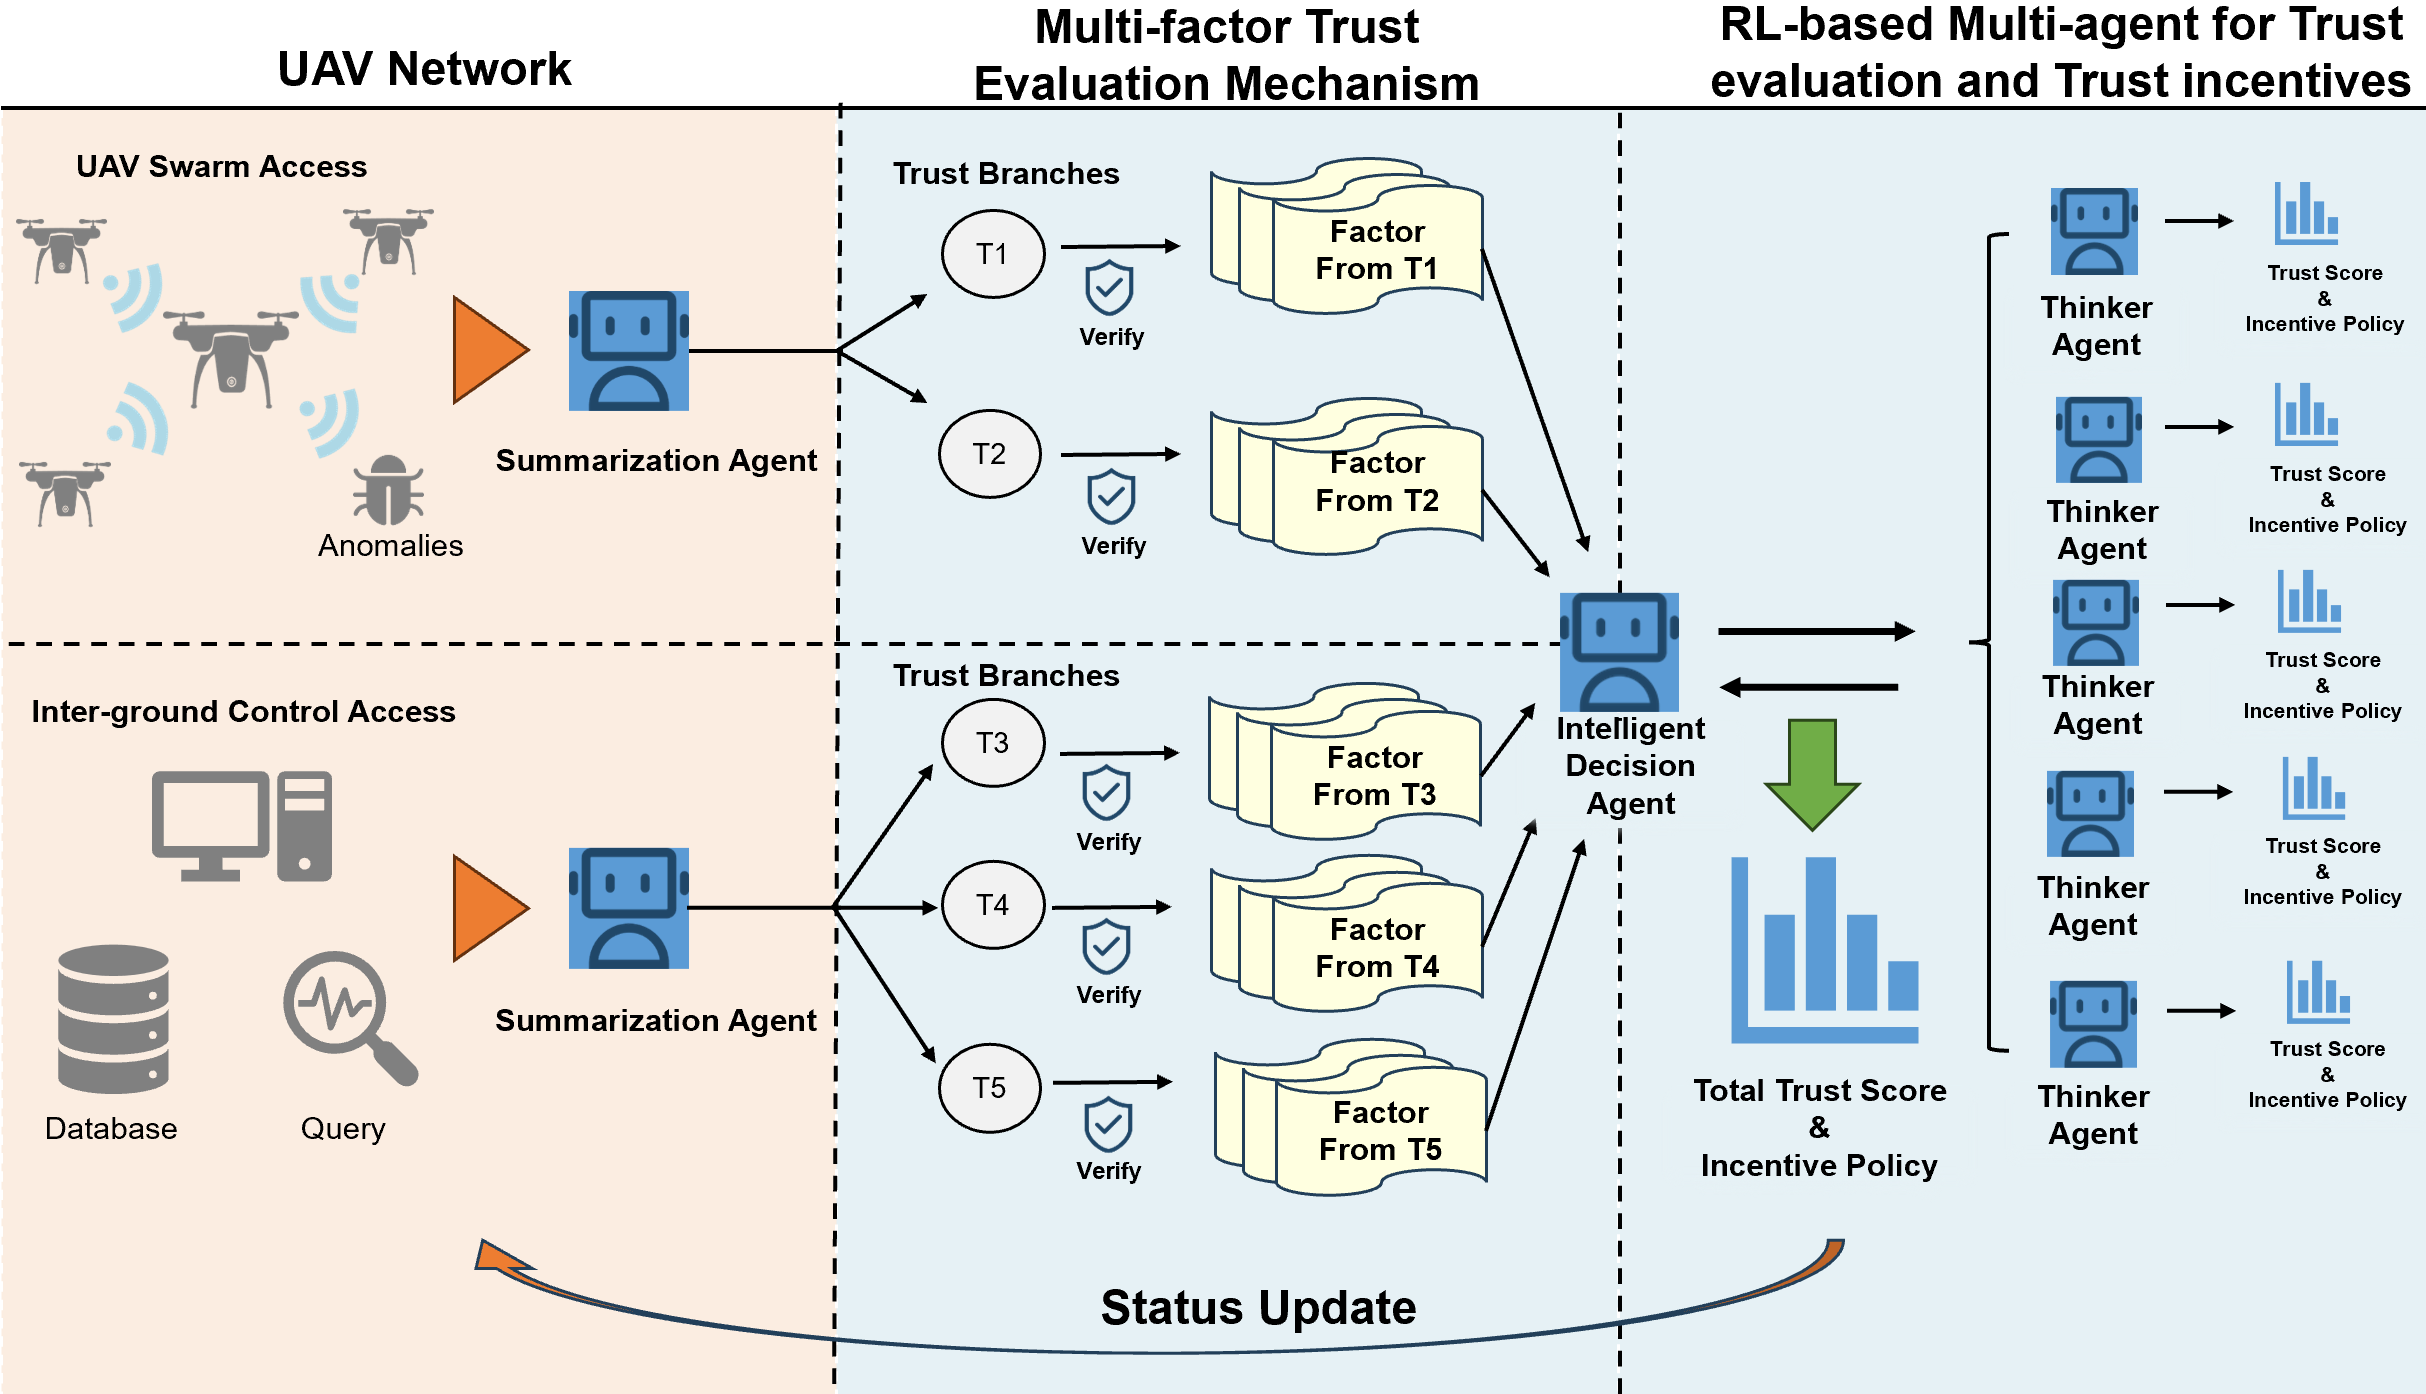
\includegraphics[width=0.85\textwidth]{ov2.png}
\caption{Intended MTIM deployment architecture. The released artifact implements the T1--T5 trust-stream features, a shared supervised network, and a model-based allocation proxy. Parallel on-board agents, confidence-weighted fusion, and a closed deployment feedback loop remain design elements rather than experimentally validated components.}
\label{fig:Proposed}
\end{figure}

\subsection{UAV Network Model}
\label{sec:net_model}
We model the low-altitude UAV network as a dynamic ad hoc network of $N$ heterogeneous UAV nodes, $\mathcal{U} = \{U_1, U_2, \dots, U_N\}$. Each node $U_i$ is characterized by a tuple $\langle \mathbf{p}_i(t), v_i(t), E_i(t), C_i \rangle$, where $\mathbf{p}_i(t) \in \mathbb{R}^2$ is the 2D position at time $t$, $v_i(t) \in [v_{\min}, v_{\max}]$ is the velocity, $E_i(t) \in [0, E_i^{\max}]$ is the residual energy, and $C_i$ denotes the computational capacity (CPU cycles/s). Nodes may enter or leave the swarm during the mission according to operational requirements.

The communication topology is a time-varying undirected graph $G(t) = (\mathcal{U}, \mathcal{E}(t))$, where an edge $(i,j) \in \mathcal{E}(t)$ exists iff the Euclidean distance satisfies $d_{ij}(t) = \|\mathbf{p}_i(t) - \mathbf{p}_j(t)\|_2 \leq R_{\text{comm}}$, with $R_{\text{comm}} = 300$~m (Table~\ref{tab:arch_params}). Each link $(i,j)$ has a time-varying quality characterized by packet delivery ratio $\text{PDR}_{ij}(t)$, received signal strength $\text{RSSI}_{ij}(t)$, and one-way latency $L_{ij}(t)$. The network is \emph{infrastructure-scarce}: no fixed base stations or ground controllers are assumed to be continuously reachable; all trust computation and decision-making must execute on-board or via peer-to-peer exchange.

\subsection{Threat Model}
\label{sec:threat_model}
We use a fixed-identity synthetic adversary model. It is not adaptive to the learned parameters.

\paragraph{Adversary capabilities.}
A subset of nodes $\mathcal{M} \subset \mathcal{U}$ ($|\mathcal{M}|/N \in [0.05, 0.50]$ in our experiments) is controlled by an adversary. Each malicious node $U_m \in \mathcal{M}$ can independently manipulate any subset of the five trust dimensions by:
\begin{itemize}[topsep=0pt,itemsep=0pt]
    \item \textbf{T1 (Behavioral)}: deviating from planned flight paths, skipping scheduled heartbeats, or responding inconsistently to coordination messages;
    \item \textbf{T2 (Communication)}: performing selective forwarding (dropping a fraction $p_{\text{drop}} \in [0.3, 1.0]$ of packets), injecting spurious traffic, or manipulating transmission power to create asymmetric links;
    \item \textbf{T3 (Energy)}: exhibiting anomalous consumption patterns (e.g., sudden depletion through jamming, or unusually low consumption by remaining idle during active mission phases);
    \item \textbf{T4 (Task)}: returning fabricated or degraded task results (e.g., falsified sensor readings, partial payload delivery);
    \item \textbf{T5 (Historical)}: this dimension is not directly manipulable by the adversary---it is an accumulated reputation signal maintained by MTIM---but its update is indirectly affected when the adversary manipulates T1--T4.
\end{itemize}

\paragraph{Attack strategies.}
We consider three canonical attack patterns that cover the spectrum from naive to evasive adversaries:
\begin{enumerate}[label={(\roman*)}]
    \item \textbf{Constant attack}: the malicious node exhibits adversarial behavior from $t = 0$ and maintains it throughout the mission. This models unsophisticated attackers and serves as a lower bound on detection difficulty.
    \item \textbf{Dormant attack}: the malicious node behaves honestly during an initial warm-up period ($t \leq T_{\text{warm}}$), accumulating trust, then switches to adversarial behavior. This models adversaries that attempt to evade initial screening.
    \item \textbf{On-off attack}: the malicious node toggles between honest and adversarial behavior with period $T_{\text{toggle}}$, attempting to keep its trust score near the classification boundary where decisions are most uncertain.
\end{enumerate}
In mixed-attack experiments, these patterns are assigned cyclically across malicious nodes. The artifact does not implement colluding peer reports, Sybil identities, an adaptive attacker, or training-data poisoning.

\paragraph{Adversary knowledge.}
The generated attacker knows neither the fitted parameters nor the decision threshold. Because it does not respond to model outputs, the experiments measure generalization across random seeds from one generator, not robustness to a strategic white-box adversary.

\paragraph{Design implications.}
The generator mainly tests whether temporal summaries of T1 and T4 separate the three attack profiles from benign nodes. It does not test majority collusion or Byzantine aggregation. Any deployment would still require cryptographic identity binding and an independently validated observation pipeline.

\subsection{Multi-factor Trust Evaluation Mechanism}
\label{sec:trust_eval}
MTIM represents credibility with five trust dimensions. They are not statistically independent, and the present study does not support an ``exponentially harder'' evasion claim. T5 is explicitly computed from the other four dimensions and is therefore a memory term, not a separate sensor.

\subsubsection{Trust Factor Decomposition}
T1 denotes behavioral consistency, T2 communication reliability, T3 energy behavior, and T4 task quality. T5 is an exponentially smoothed mean of T1--T4. Equations~\ref{eq:T1}--\ref{eq:T4} describe how these quantities could be obtained from telemetry. In the main experiment, however, the artifact samples normalized T1--T4 values directly from attack-dependent distributions and computes T5 from those samples; it does not simulate the raw packet, position, energy, or task variables in these equations.

As illustrated in Figure \ref{fig:Proposed}, the trust evaluation is decomposed into multiple trust branches, each corresponding to a distinct trust factor. Let the overall trust score of UAV node $i$ at time $t$ be denoted as $T_i(t) \in [0, 10]$, which is a function of five fundamental trust dimensions (the formal aggregation mechanism is presented in Section~\ref{sec:multi_factor_aggregation}),
where each trust branch $T_i^{(m)}(t) \in [0, 1]$ is defined as follows:

\begin{itemize}
    \item \textbf{T1: Behavioral Trust $T_i^{(1)}(t)$}. This factor evaluates operational consistency, including adherence to flight paths, communication regularity, and response reliability:
    \begin{equation}\label{eq:T1}
    T_i^{(1)}(t) = \frac{1}{N_b} \sum_{j=1}^{N_b} \mathbb{I}\!\left(a_{i,j}(t) = a_{i,j}^{expected}(t)\right)
    \end{equation}
    where $\mathbb{I}(\cdot)$ is the indicator function, $a_{i,j}(t)$ represents the actual action in behavior category $j$, and $a_{i,j}^{expected}(t)$ is the expected behavior. This yields $T_i^{(1)}(t) \in [0, 1]$.
\end{itemize}

\begin{itemize}
\item \textbf{T2: Communication Trust $T_i^{(2)}(t)$}. This factor assesses link quality and stability through packet delivery ratio, signal strength, and latency:
\begin{equation}\label{eq:T2}
T_i^{(2)}(t) = w_p \cdot PDR_i(t) + w_s \cdot \frac{RSSI_i(t)}{RSSI_{max}} + w_l \cdot \left(1 - \frac{L_i(t)}{L_{max}}\right)
\end{equation}
where $PDR_i(t)$, $RSSI_i(t)/RSSI_{max}$, and $1 - L_i(t)/L_{max}$ are each normalized to $[0, 1]$, and $w_p = 0.4, w_s = 0.3, w_l = 0.3$ are weighting coefficients with $w_p + w_s + w_l = 1$. Thus $T_i^{(2)}(t) \in [0, 1]$.
\end{itemize}

\begin{itemize}
\item \textbf{T3: Energy Trust $T_i^{(3)}(t)$}. This factor monitors energy-consumption patterns and remaining battery life to detect anomalies indicative of malfunction or compromise:
\begin{equation}\label{eq:T3}
T_i^{(3)}(t) = \frac{E_{remaining}(t)}{E_{initial}} \cdot \exp\left(-\alpha \cdot \left|C_i(t) - \bar{C}(t)\right|\right)
\end{equation}
where $\frac{E_{remaining}(t)}{E_{initial}} \in [0, 1]$ and the exponential term with $\alpha = 0.5$ is also bounded in $[0, 1]$, yielding $T_i^{(3)}(t) \in [0, 1]$.
\end{itemize}

\begin{itemize}
\item \textbf{T4: Task Execution Trust $T_i^{(4)}(t)$}. This factor measures the success rate and quality of task completion, such as sensing, data relaying, or payload delivery:
\begin{equation}\label{eq:T4}
T_i^{(4)}(t) = \frac{1}{N_t} \sum_{k=1}^{N_t} \left( \frac{Q_{i,k}(t)}{Q_k^{max}} \cdot \mathbb{I}(\mathrm{task\_success}) \right)
\end{equation}
where each term is normalized to $[0, 1]$, so $T_i^{(4)}(t) \in [0, 1]$.
\end{itemize}

\begin{itemize}
\item \textbf{T5: Historical Trust $T_i^{(5)}(t)$}. This factor incorporates long-term reputation scores and past behavior records to preserve temporal continuity in trust evaluation:
\begin{equation}\label{eq:T5}
T_i^{(5)}(t) = \beta \cdot T_i^{(5)}(t-1) + (1 - \beta) \cdot T_i^{inst}(t)
\end{equation}
where both the historical and instantaneous components are in $[0, 1]$, and the smoothing factor $\beta = 0.7$. Thus $T_i^{(5)}(t) \in [0, 1]$.
\end{itemize}

\subsubsection{Multi-factor Trust Aggregation}
\label{sec:multi_factor_aggregation}
Each trust branch independently computes a sub-score $T_i^{(m)}(t) \in [0, 1]$ based on real-time data streams and historical logs. These sub-scores are then aggregated into a global trust score $T_i(t) \in [0, 10]$ through a weighted fusion mechanism:
\begin{equation}\label{eq:aggregation}
T_i(t) = 10 \cdot \sum_{m=1}^{5} \omega_m(t) \cdot T_i^{(m)}(t)
\end{equation}
where the weights sum to one. The network learns an auxiliary weight head, but the released classifier computes risk directly from 13 summary features and does not use Eq.~\ref{eq:aggregation} to obtain its prediction.

\subsubsection{Cross-Validation Mechanism}
The multi-factor design ensures that no single point of failure or manipulation can compromise the overall trust decision. To enhance robustness, a \textbf{cross-validation mechanism} is implemented between trust branches. For any pair of trust factors $m$ and $n$, the consistency metric is defined as:
\begin{equation}\label{eq:consistency}
\Gamma_{m,n}(t) = \left| T_i^{(m)}(t) - T_i^{(n)}(t) \right|
\end{equation}
If $\Gamma_{m,n}(t) > \gamma_{\text{th}}$, where the cross-validation threshold $\gamma_{\text{th}} = 0.3$ (determined via sensitivity analysis over $\{0.1, 0.2, 0.3, 0.4, 0.5\}$ with $0.3$ yielding the best F-score on a validation subset), a potential inconsistency is flagged, triggering deeper inspection. For instance, even if a UAV exhibits normal communication behavior ($T_i^{(2)}(t)$ high), but shows abnormal energy depletion ($T_i^{(3)}(t)$ low), the system can still flag it as potentially compromised. This layered verification keeps trust continuously evaluated rather than assumed from any single evidence channel.

Furthermore, the framework supports \textbf{anomaly detection} through statistical analysis of trust factor deviations:
\begin{equation}\label{eq:anomaly}
\mathcal{A}_i(t) = \mathbb{I}\left( \sum_{m=1}^{5} \left( \frac{T_i^{(m)}(t) - \mu_m(t)}{\sigma_m(t)} \right)^2 > \chi^2_{\alpha,5} \right)
\end{equation}
where $\mu_m(t)$ and $\sigma_m(t)$ are the mean and standard deviation of trust factor $m$ across the swarm, $\chi^2_{\alpha,5}$ is the chi-squared threshold with 5 degrees of freedom at significance level $\alpha = 0.05$. This redundancy and diversity in trust evidence form the foundation for robust and adaptive trust management in UAV swarms, enabling the detection of sophisticated attacks that may manipulate multiple dimensions simultaneously.

\subsection{Supervised Multi-Head Risk Model and Allocation Proxy}
\label{sec:marl_formulation}
The intended architecture divides observation across local agents and forwards their estimates to a decision node. The executable artifact is simpler. It applies one shared supervised network independently to each node's diagnostic feature vector. Agent assignments do not enter the feature extractor, and neither confidence-weighted fusion nor budget projection is executed. We retain the broader formulation below to define a possible deployment target, but distinguish it from the evaluated model.

\subsubsection{Dec-POMDP Elements}
We consider a UAV swarm consisting of $N$ UAV nodes. The trust management system employs $M$ Thinker Agents, where each agent $j \in \{1, 2, \dots, M\}$ is responsible for a subset of UAV nodes. The overall system can be modeled as a Dec-POMDP (decentralized partially observable Markov decision process)~\cite{oliehoek2008optimal}:
\begin{equation}
\mathcal{G} = \langle \mathcal{S}, \mathcal{O}, \mathcal{A}, \mathcal{P}, \mathcal{R}, \gamma \rangle
\end{equation}
where $\mathcal{S}$ is the global state space, $\mathcal{O}$ is the joint observation space, $\mathcal{A}$ is the joint action space, $\mathcal{P}$ is the state transition probability, $\mathcal{R}$ is the reward function, and $\gamma \in [0, 1]$ is the discount factor.

\textbf{State Space}: The state $s \in \mathcal{S}$ at time $t$ is defined as the tuple of all UAV nodes' multi-factor trust scores:
\[
s(t) = (\mathbf{T}_1(t), \mathbf{T}_2(t), \dots, \mathbf{T}_N(t)),
\]
where $\mathbf{T}_k(t) = [T_k^{(1)}(t), T_k^{(2)}(t), T_k^{(3)}(t), T_k^{(4)}(t), T_k^{(5)}(t)]$ denotes the five-dimensional trust vector for node $k$, with each component in $[0, 1]$. The corresponding global trust score $\mathcal{T}_k(t) \in [0, 10]$ is computed by the Intelligent Decision Agent as described in Section \ref{sec:reward}.

\textbf{Observation Space}: Each Thinker Agent $j$ observes a partial view of the global state, consisting only of the local trust sub-scores for the nodes in its supervised subset $\mathcal{N}_j$: $o_j(t) = (\mathbf{T}_k(t))_{k \in \mathcal{N}_j} \cup (c_{jk}(t))_{k \in \mathcal{N}_j}$, where $c_{jk}(t)$ is the confidence score assigned by agent $j$ to its own assessment of node $k$.

\textbf{Action Space}: The action $a_j(t) \in \mathcal{A}_j$ for Thinker Agent $j$ is a hybrid parameterized action consisting of (1) a continuous trust-weight vector $\boldsymbol{\omega}_j(t) = [\omega_{j}^{(1)}(t), \dots, \omega_{j}^{(5)}(t)] \in \Delta^4$ on the probability simplex, and (2) a discrete incentive allocation vector $\boldsymbol{\pi}_j(t) = [\pi_{jk}(t)]_{k \in \mathcal{N}_j}$ specifying the incentive level for each supervised node. Incentive levels are quantized into five bins $\{-2, -1, 0, 1, 2\}$, corresponding to strong penalty, weak penalty, neutral allocation, weak reward, and strong reward. Thus, trust evaluation provides the state used to judge behavior, while the learned policy decides whether the node should be rewarded with more favorable task participation or penalized through restricted access. If a sampled incentive vector violates the cycle budget $B_{\text{total}}(t)$, incentives are projected greedily by retaining actions with the largest expected utility gain per unit cost until the budget is satisfied.

\textbf{Evaluated architecture}: Training is centralized and supervised. Simulator labels determine the risk, action, and value targets. At inference, labels are absent, but the artifact does not emulate decentralized message exchange; it evaluates all per-node feature vectors in one process.

\textbf{State Transition}: The state transition $\mathcal{P}$ is defined implicitly through the trust update equations (Eqs.~\ref{eq:decay}--\ref{eq:bayes_update}) in Section \ref{sec:state_update}, which govern how trust scores evolve based on observations, incentives, and temporal decay.

\subsubsection{Executable Multi-Head Network}
The implemented policy network uses per-node diagnostic features extracted from the post-warm-up trust streams. These features include recent weakness in T1, T2, T4, and T5; low-quantile T1/T4 evidence; low-score duration; T1/T4 amplitude and standard deviation; positive degradation slope; and directional cross-factor gaps. The same feature mapping is used by MTIM and by the learned baselines introduced in Section~\ref{sec:sim_setup}.

For node $k$, let $\mathbf{x}_k \in \mathbb{R}^{13}$ denote the standardized diagnostic feature vector. A shared encoder maps $\mathbf{x}_k$ to a hidden representation $h_k$:
\begin{equation}
h_k = f_{\theta}(\mathbf{x}_k).
\end{equation}
Four output heads are then computed:
\begin{equation}
\begin{aligned}
p_k &= \sigma(g_r(h_k)),\\
\omega_k^{(m)} &= \frac{\exp(g_{\omega}^{(m)}(h_k))}{\sum_{\ell=1}^{5}\exp(g_{\omega}^{(\ell)}(h_k))},\\
\mathbf{q}_k^{\pi} &= g_{\pi}(h_k),\\
v_k &= g_v(h_k),
\end{aligned}
\label{eq:policy_heads}
\end{equation}
where $p_k$ is the malicious-risk probability, $\boldsymbol{\omega}_k$ is an auxiliary trust-factor weight vector, $\mathbf{q}_k^{\pi}$ contains five supervised action scores, and $v_k$ is an auxiliary service-value estimate. Only $p_k$ is consumed by the released evaluation path; the auxiliary heads are trained and logged but do not determine the reported task-allocation probabilities. The local diagnostic trust score is
\begin{equation}
\hat{T}_{jk}=10(1-p_k),
\end{equation}
and a node is flagged as malicious when $p_k > 0.60$. A potential deployment could select an incentive bin as
\begin{equation}
\pi_{jk}^{raw} = \arg\max_{\ell \in \{-2,-1,0,1,2\}} q_{k,\ell}^{\pi},
\end{equation}
followed by a budget projection. That projection is not implemented in the current artifact.

\subsubsection{Supervised Training Objective}
\label{sec:reward}
Let $y_k \in \{0,1\}$ be the simulator label used during training. Let $\boldsymbol{\omega}_k^{*}$ be a heuristic weight target derived from the diagnostic features, $\pi_k^{*}$ an action target derived from $y_k$ and a risk hint, and $v_k^{*}$ a service-value target derived directly from $y_k$. The network minimizes
\begin{equation}
\begin{aligned}
\mathcal{L}(\theta) ={}& \mathrm{BCE}_{w}(y_k,p_k)
 + 0.25 \left\|\boldsymbol{\omega}_k-\boldsymbol{\omega}_k^{*}\right\|_2^2\\
&+ 0.20\,\mathrm{CE}(\pi_k^{*},\mathbf{q}_k^{\pi})
 + 0.10 \left(v_k-v_k^{*}\right)^2 .
\end{aligned}
\label{eq:implemented_loss}
\end{equation}
The primary term is weighted binary cross-entropy with a positive-class weight of 2.0. There is no reward return or temporal-difference target in Eq.~\ref{eq:implemented_loss}; the value target is $0.8$ for benign nodes and $-0.4$ for malicious nodes. The action target also depends on the ground-truth class. Training uses seeds 0--9 and a fixed decision threshold of 0.60. Evaluation seeds 1000--1049 are not used for fitting. The method is therefore a multi-task supervised classifier, not an offline or online reinforcement-learning algorithm.

The following aggregation equations specify an unevaluated extension for deployments in which several agents observe the same node. They are not invoked by the released Python evaluation.

\textbf{Total Trust Score Aggregation}: The Intelligent Decision Agent computes the total trust score $\mathcal{T}_k(t)$ for each UAV node $k$ by combining the individual trust scores from all Thinker Agents that have observed or interacted with node $k$:
\begin{equation}\label{eq:ida_global}
\mathcal{T}_k(t) = \frac{\sum_{j=1}^{M} \phi_{jk}(t) \cdot \hat{T}_{jk}(t)}{\sum_{j=1}^{M} \phi_{jk}(t)}
\end{equation}
where $\phi_{jk}(t) \in [0, 1]$ is the confidence weight assigned to Thinker Agent $j$'s assessment of node $k$, computed based on the agent's historical accuracy:
\begin{equation}\label{eq:ida_weight}
\phi_{jk}(t) = \frac{\exp\left(-\gamma \cdot \varepsilon_{jk}(t)\right)}{\sum_{j'=1}^{M} \exp\left(-\gamma \cdot \varepsilon_{j'k}(t)\right)}
\end{equation}
with $\varepsilon_{jk}(t) = \frac{1}{t} \sum_{\tau=1}^{t} \left| \hat{T}_{jk}(\tau) - T_{jk}^{obs}(\tau) \right|$ representing the mean absolute error of agent $j$ for node $k$ over time, and $\gamma = 2.0$ a scaling parameter.

\textbf{Dispersion measure}: A deployment may quantify disagreement among local estimates as
\begin{equation}\label{eq:ida_uncertainty}
\sigma_k^2(t) = \frac{\sum_{j=1}^{M} \phi_{jk}(t) \left( \hat{T}_{jk}(t) - \mathcal{T}_k(t) \right)^2}{\sum_{j=1}^{M} \phi_{jk}(t)} + \sigma_0^2
\end{equation}
where $\sigma_0^2 = 0.1$ is a variance floor. This weighted dispersion is not a Bayesian posterior variance unless a probabilistic observation model is supplied.

\textbf{Final Trust Classification}: Based on the total trust score and uncertainty, the Intelligent Decision Agent classifies nodes into trust categories:
\begin{equation}\label{eq:ida_classification}
C_k(t) =
\begin{cases}
\text{Trusted} & \text{if } \mathcal{T}_k(t) \geq \theta_{\text{high}} \text{ and } \sigma_k(t) \leq \sigma_{\text{th}} \\
\text{Suspicious} & \text{if } \theta_{\text{low}} \leq \mathcal{T}_k(t) < \theta_{\text{high}} \text{ or } \sigma_k(t) > \sigma_{\text{th}} \\
\text{Malicious} & \text{if } \mathcal{T}_k(t) < \theta_{\text{low}} \text{ and } \sigma_k(t) \leq \sigma_{\text{th}}
\end{cases}
\end{equation}
where $\theta_{\text{high}}$ and $\theta_{\text{low}}$ are trust thresholds, and $\sigma_{\text{th}}$ is the uncertainty threshold.

A future decision node could map global trust assessments to resource-allocation actions:
\begin{equation}\label{eq:incentive_policy}
\boldsymbol{\Pi}(t) = \left\{ \pi_{jk}(t) : j \in [1, M], k \in \mathcal{N}_j \right\},
\end{equation}
where $\pi_{jk}(t) \in \mathcal{A}_{\text{inc}} = \{-2, -1, 0, 1, 2\}$ is the incentive action for node $k$ by agent $j$, encoding strong penalty ($-2$) through strong reward ($+2$). The policy is determined by solving a constrained optimization that maximizes expected network-wide utility:
\begin{equation}\label{eq:incentive_opt}
\max_{\boldsymbol{\Pi}(t)}\; \mathbb{E}\left[ \sum_{k=1}^{N} U_k\!\left( \mathcal{T}_k(t), \pi_{\cdot k}(t) \right) \right],
\end{equation}
subject to the budget constraint $\sum_{j=1}^{M} \sum_{k \in \mathcal{N}_j} c(\pi_{jk}(t)) \leq B_{\text{total}}(t)$, where $c(\pi) = |\pi|$ quantifies the resource cost of each incentive action. The per-node utility function is:
\begin{equation}\label{eq:utility}
U_k\!\left( \mathcal{T}_k(t), \pi_{\cdot k}(t) \right) = \mathcal{T}_k(t) \cdot \bigl(1 + \delta \cdot \mathbb{I}(\pi_{\cdot k}(t) > 0)\bigr) - \kappa \cdot \mathbb{I}\bigl(\mathcal{T}_k(t) < \theta_{\text{low}}\bigr),
\end{equation}
with $\delta = 0.2$ and $\kappa = 2.0$. These equations are design specifications. The current task-success simulator instead converts each method's score to a sampling weight and applies a stronger down-weighting rule to MTIM; it does not solve Eq.~\ref{eq:incentive_opt}.

\subsubsection{State Update Mechanism for Trust Evolution}
\label{sec:state_update}
The following state update is a proposed deployment mechanism, not the recurrence used in the main generator. In the artifact, T5 follows $T_5(t)=0.84T_5(t-1)+0.16\bar{T}_{1:4}(t)$ and the trained risk model is evaluated on summary windows. Incentive outputs do not alter later trust streams. A possible deployment transition is
\begin{equation}
\mathbf{T}(t+1) = f\left( \mathbf{T}(t), \mathbf{A}^{inc}(t), \mathbf{A}^{task}(t), \mathbf{E}(t) \right)
\end{equation}
where $\mathbf{T}(t) \in \mathbb{R}^N$ is the vector of global trust scores, $\mathbf{A}^{inc}(t)$ is the incentive action matrix, $\mathbf{A}^{task}(t)$ captures task execution outcomes, and $\mathbf{E}(t)$ represents environmental factors. The trust score for each node $k$ evolves according to the following three-stage process:

\textbf{Temporal Trust Decay}: To prevent trust stagnation and enforce continuous verification, we incorporate a temporal decay factor:
\begin{equation}\label{eq:decay}
\tilde{\mathcal{T}}_k(t+1) = \mathcal{T}_k(t) \cdot \exp\left(-\rho \cdot \Delta t\right)
\end{equation}
where $\rho = 0.01$ is the decay rate (see Table~\ref{tab:arch_params}) and $\Delta t = 10$~s is the trust update interval. This ensures that trust gradually diminishes without positive reinforcement.

\textbf{Trust Update Based on Observations}: The final trust score is updated via a Bayesian filter that combines the decayed prior with new observations:
\begin{equation}\label{eq:bayes_update}
\begin{aligned}
  \mathcal{T}_k(t+1) ={}& a_k(t)\,\tilde{\mathcal{T}}_k(t+1)
  + \bigl(1-a_k(t)\bigr)\\
  &\cdot T_k^{obs}(t+1),\\
  a_k(t) ={}& \frac{\sigma_{obs}^2}{\sigma_k^2(t)+\sigma_{obs}^2}.
\end{aligned}
\end{equation}
where $\sigma_{obs}^2 = 0.5$ is the observation noise variance, and $T_k^{obs}(t+1)$ is the aggregated observed trust score from all Thinker Agents. This form assigns more weight to new observations when the prior uncertainty $\sigma_k^2(t)$ is high, and more weight to the decayed prior when the current estimate is confident. The observation term is:
\begin{equation}\label{eq:obs_aggregation}
T_k^{obs}(t+1) = \frac{1}{|\mathcal{M}_k(t+1)|} \sum_{j \in \mathcal{M}_k(t+1)} T_{jk}^{obs}(t+1)
\end{equation}
with $\mathcal{M}_k(t+1)$ denoting the set of agents that observed node $k$ at time $t+1$.

\textbf{Boundedness and Empirical Stability}: The trust update mechanism in Eqs.~\ref{eq:decay}--\ref{eq:bayes_update} admits bounded updates under the $[0, 10]$ trust scale. Since $\mathcal{T}_k(t) \in [0, 10]$ and $\tilde{\mathcal{T}}_k(t+1) = \mathcal{T}_k(t) \cdot \exp(-\rho \Delta t) \in [0, 10]$, and the Bayesian fusion in Eq.~\ref{eq:bayes_update} is a convex combination of two bounded terms (with coefficients in $[0, 1]$ that sum to one), the trust score remains in $[0, 10]$ for all $t$, preventing numerical divergence.

We do not claim convergence of the Dec-POMDP or of the generated trajectories. The boundedness argument applies only to the proposed convex update.

\textbf{Scope of the update claim}: Equations~\ref{eq:decay}--\ref{eq:bayes_update} show boundedness of the proposed update only. They do not establish convergence, and the released simulator does not close the action-to-future-state loop.

\begin{figure}[!htbp]
\centering
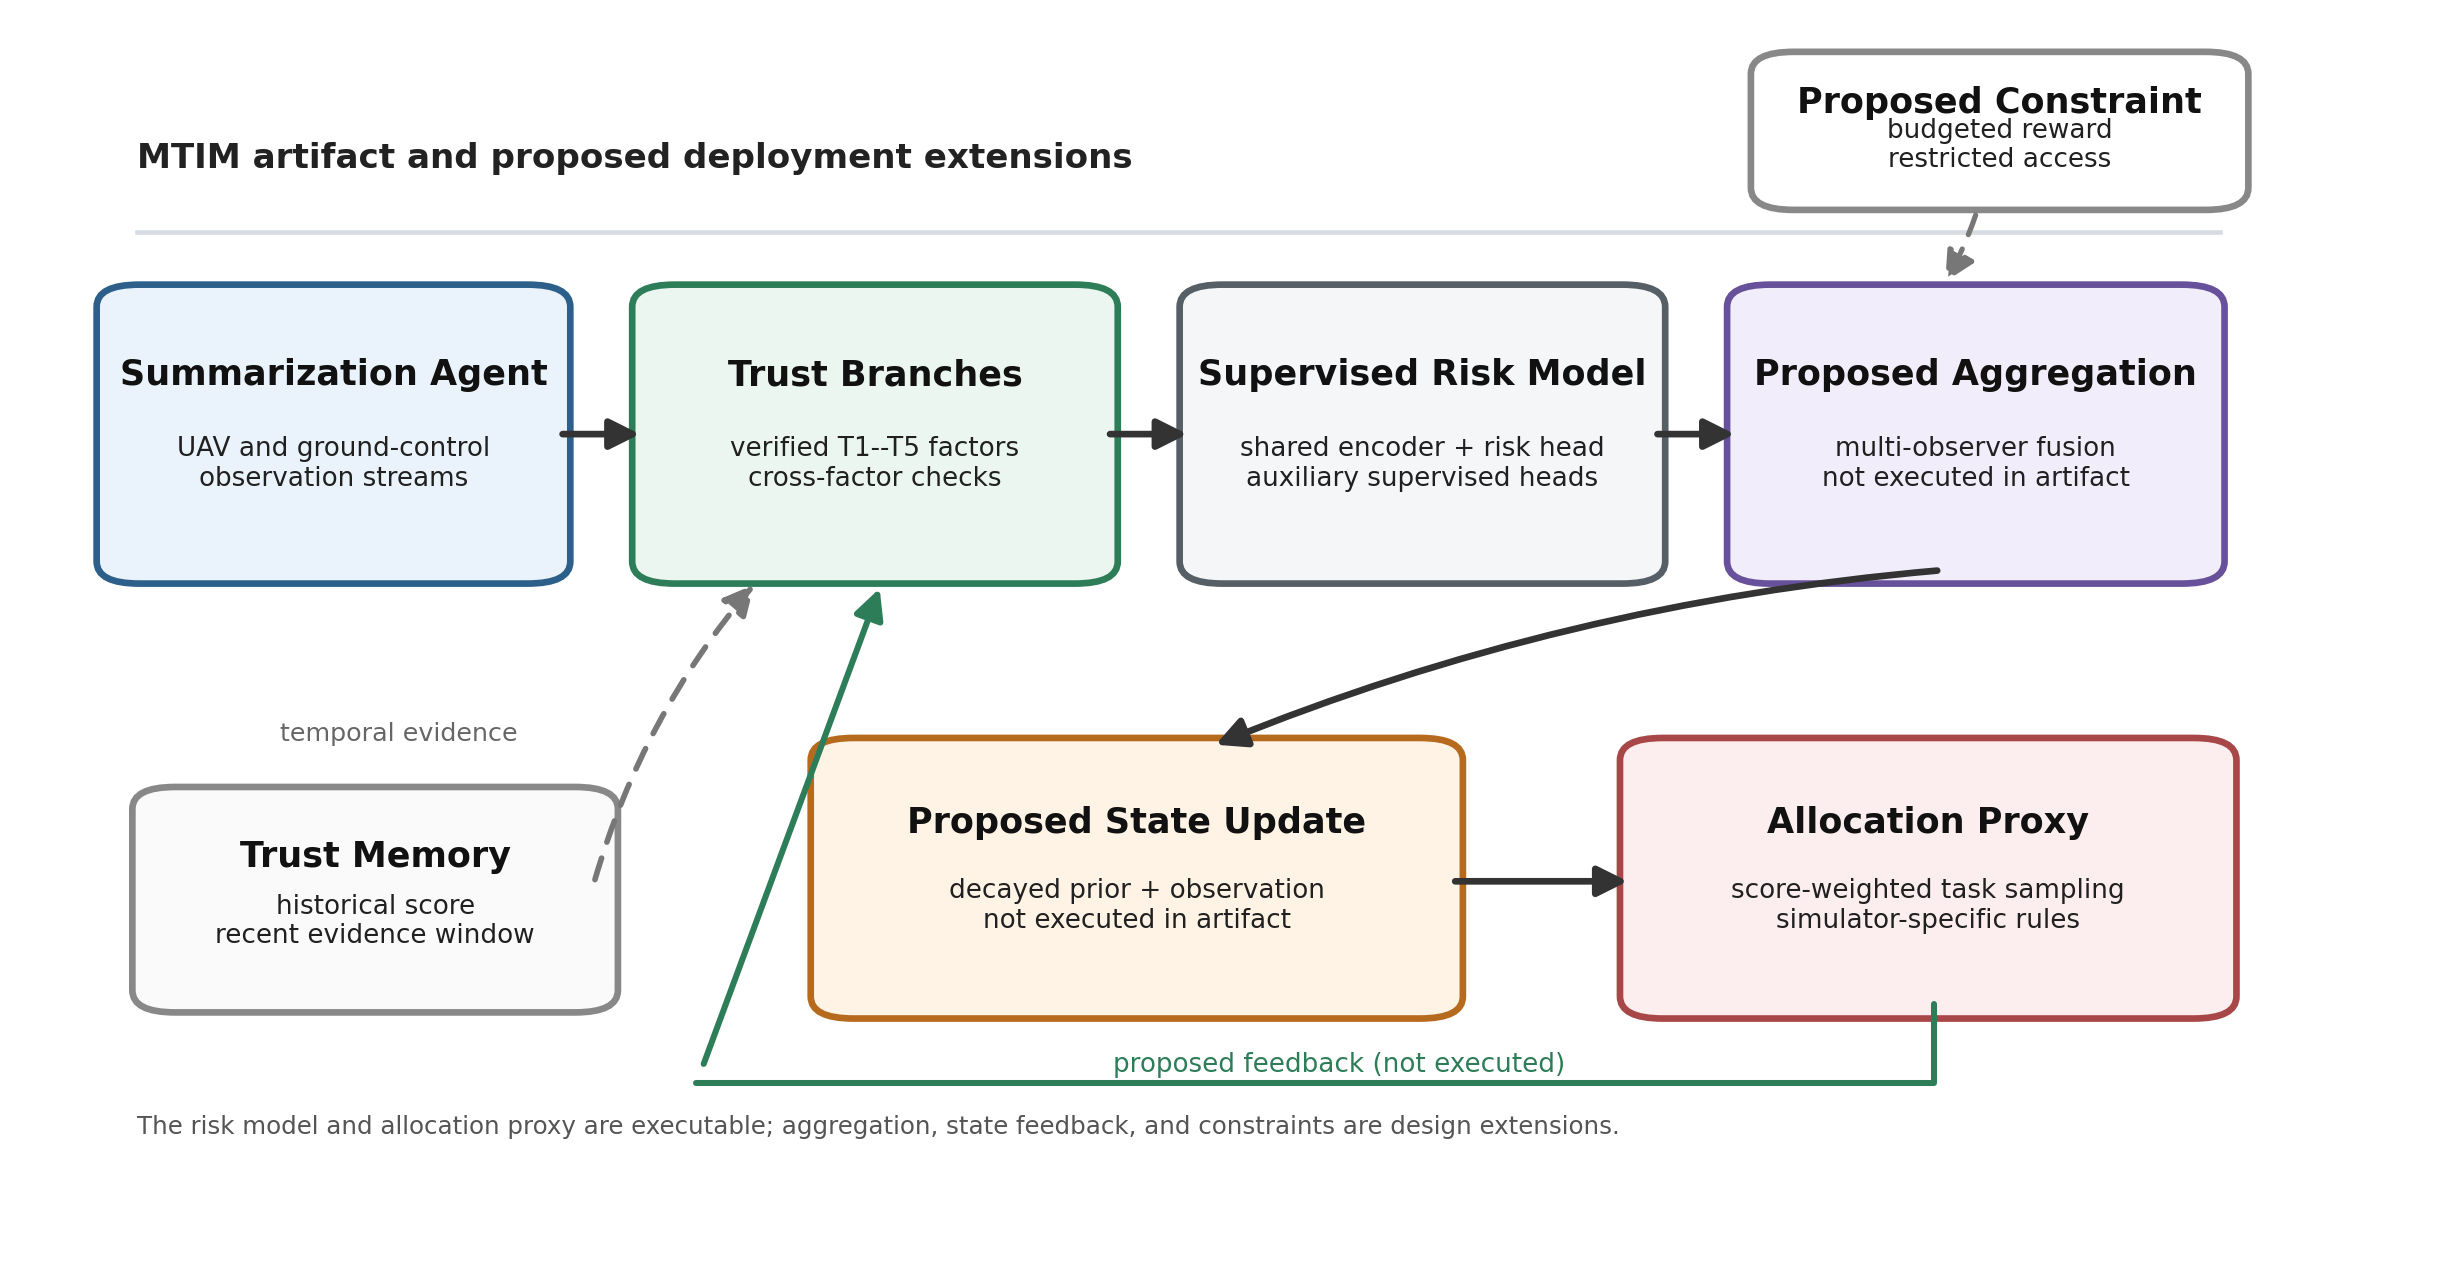
\includegraphics[width=\textwidth]{update.png}
\caption{Proposed state-update and allocation loop. Solidly implemented elements in the artifact are trust-stream generation, feature extraction, risk inference, and a task-allocation proxy. Confidence fusion, budgeted incentives, and action-dependent future trust remain unvalidated extensions.}
\label{fig:update}
\end{figure}

\subsubsection{Evaluation Metrics}
This section defines the main evaluation metrics used throughout the experiments. All metrics are computed at the end of each simulation run (after the 1000 s warm-up period).

\textbf{Trust Classification Metrics}: For malicious-node detection, the confusion matrix is defined over the three-class output of Eq.~\ref{eq:ida_classification}, with Suspicious mapped to Malicious for binary evaluation. Let TP, TN, FP, FN denote true/false positives/negatives, respectively. Detection accuracy, precision, recall, and F$_1$-score are:
\begin{equation}\label{eq:accuracy}
\begin{aligned}
\mathrm{Accuracy} = \frac{\mathrm{TP} + \mathrm{TN}}{\mathrm{TP} + \mathrm{TN} + \mathrm{FP} + \mathrm{FN}},
&\qquad
\mathrm{Precision} = \frac{\mathrm{TP}}{\mathrm{TP} + \mathrm{FP}},
\\
\mathrm{Recall} = \frac{\mathrm{TP}}{\mathrm{TP} + \mathrm{FN}},
&\qquad
F_1 = \frac{2 \cdot \mathrm{Precision} \cdot \mathrm{Recall}}{\mathrm{Precision} + \mathrm{Recall}}.
\end{aligned}
\end{equation}
Ground-truth labels are assigned at simulation initialization according to the attack model (Section~\ref{sec:threat_model}) and are never observable by the Thinker Agents during execution.

\textbf{Mission-Level Metric}: The task success rate (TSR) measures mission continuity independently of detection accuracy:
\begin{equation}\label{eq:tsr}
\mathrm{TSR} = N_{\mathrm{succ}} \,/\, N_{\mathrm{all}},
\end{equation}
In the artifact, each trial samples 220 single-node assignments. A benign selection succeeds with base probability 0.90 and a malicious selection with 0.30, followed by a small score adjustment. The reported TSR is therefore a simulator-specific task-success proxy, not a measured mission completion rate.

\textbf{Resource-model outputs}: Communication overhead and evaluation latency are generated from method-specific affine formulas plus Gaussian noise. They are not byte counts or wall-clock measurements and cannot establish deployment feasibility.

\subsubsection{Algorithm Summary}
Table~\ref{alg:mtim} consolidates the MTIM trust evaluation and incentive loop for a single update cycle.

\begin{table}[!htbp]
\centering
\caption{MTIM trust evaluation and incentive cycle for one update interval $\Delta t$.}
\label{alg:mtim}
\footnotesize
\begin{tabularx}{\textwidth}{@{}rX@{}}
\toprule
\multicolumn{2}{@{}l}{\textbf{Input:} Current trust vectors $\{\mathbf{T}_k(t)\}_{k=1}^{N}$ and agent assignments $\{\mathcal{N}_j\}_{j=1}^{M}$.}\\
\multicolumn{2}{@{}l}{\textbf{Output:} Global trust scores $\{\mathcal{T}_k(t)\}_{k=1}^{N}$, classifications $\{C_k(t)\}_{k=1}^{N}$, and incentives $\{\pi_{jk}(t)\}$.}\\
\midrule
1 & For each Thinker Agent $j = 1,\dots,M$, collect local observations $o_j(t)=\{\mathbf{T}_k(t)\}_{k\in\mathcal{N}_j}$.\\
2 & Extract diagnostic features and compute $p_k$ and auxiliary heads using the frozen network in Eq.~\ref{eq:policy_heads}.\\
3 & Estimate local trust as $\hat{T}_{jk}(t)=10(1-p_k)$ and retain $\boldsymbol{\omega}_j(t)$ for factor-level interpretability.\\
4 & Apply the cross-validation check in Eq.~\ref{eq:consistency} and flag inconsistent nodes.\\
5 & Classify nodes at the fixed risk threshold $p_k>0.60$.\\
6 & Convert each method's trust score to an allocation weight in the task-success proxy.\\
7 & Sample tasks and log classification and proxy outcomes.\\
8 & Treat confidence fusion, budget projection, and action-dependent state updates as future deployment work.\\
\bottomrule
\end{tabularx}
\end{table}

%%%%%%%%%%%%%
\section{Performance Evaluation}
\label{sec:evaluation}

Our evaluation targets four questions:
\begin{enumerate}[label={(\textbf{Q\arabic*})},leftmargin=*]
    \item \textbf{In-generator detection:} How accurately does the model classify nodes drawn from the same trust-stream generator on held-out seeds?
    \item \textbf{Allocation proxy:} What task-success values arise under the simulator's score-to-selection rules?
    \item \textbf{Feature dependence:} Which temporal summaries are associated with the result?
    \item \textbf{External check:} Does the ranking persist on the bundled ns-3-derived trace?
\end{enumerate}

\subsection{Simulation Setup}
\label{sec:sim_setup}

\paragraph{Implementation.}
The evaluation uses a reproducible trust-stream generator and a supervised PyTorch network. All methods consume the same normalized T1--T5 arrays. FUBA, GALTrust, and GDM-DTM are local adapters rather than the original implementations. A separate converter is exercised on one ns-3-derived trace.

\paragraph{Network and mobility.}
The main generator runs for 500 steps at a nominal 10~s interval. It samples T1--T4 directly from fixed benign and attack-dependent means, adds Gaussian noise and node bias, and updates T5 recursively. Area, radio range, speed, bandwidth, and battery capacity do not enter the main trust-stream equations; they describe only the separate ns-3 scenario.

\paragraph{Adversary configuration.}
Malicious nodes implement the three attack strategies defined in Section~\ref{sec:threat_model}: constant (adversarial from $t=0$), dormant (switch to adversarial at $t = T_{\text{warm}} + \Delta$, where $\Delta \sim \mathcal{U}(200, 500)$~s), and on-off (toggle with period $T_{\text{toggle}} = 500$~s). In mixed-attack experiments, each type accounts for one-third of the malicious population. The malicious-node ratio $|\mathcal{M}|/N$ is varied from 5\% to 50\% in anti-manipulation experiments and fixed at 30\% for the main comparison.

\paragraph{Training protocol.}
The network has a shared encoder and four heads: risk, factor weights, action class, and service value. All targets are supervised or heuristic. Seeds 0--9 produce 450 node-level training samples; evaluation uses seeds 1000--1049. The fixed threshold is 0.60. Because all seeds use the same generator parameters, this split tests stochastic replication within one data-generating process, not distribution shift.

\paragraph{Evaluation protocol.}
Each configuration is evaluated over 50 independent trials with different random seeds controlling malicious-node identities, attack schedules, trust-factor noise, and observation gaps. Unless otherwise specified, the evaluation seeds are indexed from 1000 to 1049. All reported results are computed from the trained execution policy and fixed baseline thresholds, and are reported as mean $\pm$ standard deviation.

\begin{table}[!htbp]
  \setlength{\abovecaptionskip}{3pt}
  \setlength{\belowcaptionskip}{6pt}
  \setlength{\tabcolsep}{5pt}
  \centering
  \caption{Executable trust-stream and training parameters.}
  \label{tab:arch_params}
  \scalebox{0.92}{
  \begin{tabular}{lcl}
    \toprule
    \textbf{Category} & \textbf{Parameter} & \textbf{Value} \\
    \midrule
    \multirow{4}{*}{Generator}
      & Steps / nominal interval & 500 / 10~s \\
      & Warm-up & 100 steps \\
      & UAV count $N$ & 5--50 (default: 15) \\
      & Trust-stream noise & Gaussian, $\sigma=0.10$ \\
    \midrule
    \multirow{3}{*}{Attacks}
      & Types & constant, dormant, on--off \\
      & Main malicious ratio & 30\% \\
      & Ratio grid & 5--50\% \\
    \midrule
    \multirow{5}{*}{Training}
      & Network & PyTorch supervised multi-head MLP \\
      & Training seeds & 0--9 \\
      & Evaluation seeds & 1000--1049 \\
      & Decision threshold & 0.60 (fixed before held-out evaluation) \\
      & Python dependencies & numpy, pandas, matplotlib, scipy, torch \\
    \bottomrule
  \end{tabular}}
\end{table}

\paragraph{Baselines.}
We compare MTIM against six methods spanning the design spectrum from naive fusion to learned trust classification:

\begin{itemize}[topsep=0pt,itemsep=2pt]
    \item \textbf{MFA (Multi-factor Average)}: Equal-weighted average of T1--T5, representing the performance floor achievable without any learning or adaptation. Included to isolate the gain attributable to adaptive weighting.
    \item \textbf{FUBA}~\cite{benfriha2024fuba}: Fuzzy logic-based trust analytics for FANETs, reimplemented as membership-function trust fusion over the shared T1--T5 stream.
    \item \textbf{GALTrust}~\cite{akram2024galtrust}: Generative-adversarial trust management, reimplemented as a distance-to-honest-profile anomaly score with volatility and consistency terms over the same stream.
    \item \textbf{GDM-DTM}~\cite{hu2025gdm}: Group decision-making dynamic trust management, reimplemented as weighted group-decision trust fusion with a consistency penalty.
    \item \textbf{LR-Trust}: A logistic risk classifier trained on exactly the same diagnostic features and training seeds as MTIM, but without MTIM's trust-weight, incentive, or value heads.
    \item \textbf{MLP-Trust}: A two-layer neural risk classifier trained on exactly the same diagnostic features and training seeds as MTIM, but without MTIM's trust-weight, incentive, or value heads.
\end{itemize}

All baselines share the identical generated trust-factor streams and ground-truth labels as MTIM. Because official source code and original feature pipelines for FUBA, GALTrust, and GDM-DTM are not bundled, those baseline results should be interpreted as paper-level reimplementations under a common T1--T5 interface, not as definitive re-evaluations of the original authors' implementations. LR-Trust and MLP-Trust are added specifically to test whether MTIM's advantage persists against stronger learned classifiers with identical input information.

\paragraph{Comparison and statistical protocol.}
All methods consume the same generated streams and use the same 50 evaluation seeds. MTIM, LR-Trust, and MLP-Trust use the same feature vectors. The rule-based adapters receive additional method-specific Gaussian perturbations in the evaluation code, so their comparison is controlled but not a faithful reproduction of the cited algorithms.

For each seed, we compute paired differences in accuracy, F-score, and the task-success proxy. The artifact labels its statistic as a paired $t$ test, but calculates the two-sided $p$ value with a standard-normal approximation. We apply Holm correction across 18 comparisons. Accuracy and F-score do not differ significantly between MTIM and MLP-Trust. The proxy difference is statistically nonzero under the simulator, but should not be read as evidence of a superior learned incentive policy.

\begin{table}[!htbp]
  \centering
  \caption{Performance comparison of MTIM with baseline methods under the unified experimental setting (30\% malicious-node ratio, 15 UAVs, 5000 s simulation). All values are mean $\pm$ standard deviation over 50 independent trials.}
  \label{tab:baseline_comparison}
  \footnotesize
  \setlength{\tabcolsep}{6pt}
  \renewcommand{\arraystretch}{1.15}
  \resizebox{\textwidth}{!}{%
  \begin{tabular}{l c c c c c}
    \toprule
    Method & Accuracy & F-score & TSR proxy & Cost model (KB/UAV) & Time model (ms) \\
    \midrule
    MFA & 80.3\% $\pm$ 10.5\% & 69.4\% $\pm$ 16.3\% & 79.7\% $\pm$ 4.8\% & 11.3 $\pm$ 1.8 & 10.2 $\pm$ 4.5 \\
    FUBA \cite{benfriha2024fuba} & 84.1\% $\pm$ 9.2\% & 76.1\% $\pm$ 14.6\% & 82.5\% $\pm$ 4.2\% & 16.7 $\pm$ 1.7 & 17.1 $\pm$ 4.1 \\
    GALTrust \cite{akram2024galtrust} & 76.1\% $\pm$ 6.0\% & 41.7\% $\pm$ 21.8\% & 75.7\% $\pm$ 4.2\% & 31.4 $\pm$ 1.8 & 40.6 $\pm$ 4.0 \\
    GDM-DTM \cite{hu2025gdm} & 85.1\% $\pm$ 8.3\% & 77.3\% $\pm$ 12.6\% & 81.3\% $\pm$ 3.9\% & 19.4 $\pm$ 1.7 & 21.5 $\pm$ 3.7 \\
    LR-Trust & 88.1\% $\pm$ 9.6\% & 81.5\% $\pm$ 15.4\% & 87.6\% $\pm$ 3.6\% & 21.3 $\pm$ 1.8 & 24.5 $\pm$ 3.7 \\
    MLP-Trust & \textbf{94.7\%} $\pm$ 5.6\% & \textbf{92.1\%} $\pm$ 7.9\% & \underline{88.3\%} $\pm$ 3.9\% & 25.2 $\pm$ 2.0 & 36.1 $\pm$ 3.6 \\
    MTIM (ours) & \underline{94.4\%} $\pm$ 5.6\% & \underline{91.8\%} $\pm$ 8.0\% & \textbf{90.5\%} $\pm$ 3.7\% & 34.0 $\pm$ 1.8 & 58.3 $\pm$ 4.3 \\
    \bottomrule
  \end{tabular}}
\end{table}

\noindent\footnotesize{TSR is a model-based proxy. The cost and time columns are outputs of affine formulas with injected noise; they are not measurements. Under Holm correction, MTIM's Accuracy and F-score differ from the rule adapters and LR-Trust, but not from MLP-Trust.}
\normalsize

\paragraph{Analysis of Table~\ref{tab:baseline_comparison}.}
MTIM achieves 94.4\% accuracy, a 91.8\% F-score, and a 90.5\% task-success proxy. Three observations delimit the result:

\textbf{(i) Temporal features fit the generator.} MFA reaches 80.3\% accuracy, FUBA 84.1\%, and GDM-DTM 85.1\%. The learned models exploit low-quantile and slope features that closely match how dormant and on--off attacks are generated. This is an in-distribution advantage, not evidence of robustness to unseen attack mechanisms.

\textbf{(ii) Strong learned baselines narrow the detection claim.} LR-Trust improves over non-neural fusion baselines but still trails MTIM by 6.3~pp in accuracy. MLP-Trust reaches 94.7\% accuracy and 92.1\% F-score, which are statistically indistinguishable from MTIM's 94.4\% and 91.8\%. Thus, the evidence does not support claiming that MTIM is a strictly better detector than a strong neural risk classifier with the same features; the stronger claim is that MTIM links comparable detection quality to better mission-level action.

\textbf{(iii) The allocation result is confounded by simulator rules.} MTIM's proxy is 2.2~pp above MLP-Trust, but the task simulator down-weights nodes predicted malicious more strongly for MTIM and adds 0.02 to benign MTIM assignments. The reported incentive head is not used in this calculation. The difference therefore cannot be attributed to learned incentive coupling.

\noindent\textbf{Overhead trade-off.}\par
\noindent
The values in the last two columns are generated by \texttt{resource\_metrics}; no packets are serialized and no inference path is timed. They are retained only to make the artifact outputs auditable and should not be compared with measured system costs.

\paragraph{Robustness across malicious-node ratios.}
Table~\ref{tab:multi_ratio} reports accuracy and TSR at 10\%, 30\%, and 50\% malicious-node ratios. MTIM retains the best TSR across all three ratios. For detection accuracy, MTIM and MLP-Trust are closely matched: MLP-Trust is slightly higher at 10\% and 30\%, whereas MTIM is higher at 50\%. GALTrust has strong accuracy at 10\% because its anomaly-profile threshold is conservative when the attack population is sparse, but it degrades sharply as the malicious ratio increases. MTIM's accuracy remains between 94.4\% and 96.8\%, while TSR remains above 88\%, indicating that the trained policy continues to support mission-level decisions under dense adversarial pressure. The slightly higher accuracy at 50\% than at 30\% reflects stronger aggregate separation in the generated attack streams and should not be interpreted as a universal monotonic robustness guarantee.

\begin{table}[!htbp]
  \centering
  \caption{Detection accuracy and TSR at three malicious-node ratios ($N = 15$, 50 trials). Best values in \textbf{bold}, second-best \underline{underlined}.}
  \label{tab:multi_ratio}
  \footnotesize
  \setlength{\tabcolsep}{5pt}
  \renewcommand{\arraystretch}{1.15}
  \begin{tabular}{l c c c c c c}
    \toprule
    \multirow{2}{*}{Method} & \multicolumn{2}{c}{10\% Malicious} & \multicolumn{2}{c}{30\% Malicious} & \multicolumn{2}{c}{50\% Malicious} \\
    \cmidrule(lr){2-3} \cmidrule(lr){4-5} \cmidrule(lr){6-7}
    & Accuracy & TSR & Accuracy & TSR & Accuracy & TSR \\
    \midrule
    MFA & 86.1 $\pm$ 9.5 & 87.4 $\pm$ 3.1 & 80.3 $\pm$ 10.5 & 79.7 $\pm$ 4.8 & 76.9 $\pm$ 8.2 & 71.1 $\pm$ 4.9 \\
    FUBA & 83.7 $\pm$ 9.8 & 87.8 $\pm$ 3.3 & 84.1 $\pm$ 9.2 & 82.5 $\pm$ 4.2 & 81.1 $\pm$ 9.7 & 73.8 $\pm$ 5.2 \\
    GALTrust & \underline{91.2} $\pm$ 4.4 & 85.2 $\pm$ 3.2 & 76.1 $\pm$ 6.0 & 75.7 $\pm$ 4.2 & 63.7 $\pm$ 7.6 & 65.3 $\pm$ 3.8 \\
    GDM-DTM & 87.2 $\pm$ 7.9 & 88.5 $\pm$ 2.3 & 85.1 $\pm$ 8.3 & 81.3 $\pm$ 3.9 & 82.4 $\pm$ 7.8 & 73.9 $\pm$ 4.5 \\
    LR-Trust & 90.4 $\pm$ 7.4 & 90.2 $\pm$ 2.0 & 88.1 $\pm$ 9.6 & 87.6 $\pm$ 3.6 & 88.1 $\pm$ 8.1 & 85.3 $\pm$ 4.6 \\
    MLP-Trust & \textbf{97.3} $\pm$ 4.3 & \underline{90.6} $\pm$ 2.0 & \textbf{94.7} $\pm$ 5.6 & \underline{88.3} $\pm$ 3.9 & \underline{94.4} $\pm$ 5.1 & \underline{85.6} $\pm$ 5.3 \\
    MTIM (ours) & \underline{96.8} $\pm$ 4.5 & \textbf{92.6} $\pm$ 1.9 & \underline{94.4} $\pm$ 5.6 & \textbf{90.5} $\pm$ 3.7 & \textbf{95.5} $\pm$ 4.4 & \textbf{88.8} $\pm$ 4.6 \\
    \bottomrule
  \end{tabular}
\end{table}

\paragraph{Policy fitting stability.}
On training seeds 0--9, the final MTIM policy reaches 100.0\% training accuracy and F-score at threshold 0.60, with mean malicious risk 0.9997 and mean benign risk 0.0004. This complete training-set separation indicates that the generated training streams are highly learnable, so the reported performance is based on held-out seeds 1000--1049 rather than training metrics. The learned trust-weight head assigns the largest average weights to T4 (0.323) and T1 (0.314), followed by T2 (0.145), T5 (0.137), and T3 (0.081), matching the threat model in which sustained task/behavior degradation is harder for evasive attackers to hide than energy behavior.

\subsection{Trust Evolution Analysis}
\label{sec:trust_evolution}
Figure~\ref{fig:trust_value_evolution} tracks the diagnostic trust index from the post-warm-up phase to 5000~s under $M \in \{2,5,10\}$. The curves are recomputed by repeatedly truncating each generated stream and applying the same fitted model. Because $M$ affects the generator's random seed but does not enter the policy features, these curves do not isolate an agent-count effect.

Benign nodes remain mostly above 8.0, while malicious nodes decline as low-quantile and slope evidence accumulates. Differences among the three $M$ curves may reflect different random streams and should not be interpreted as an aggregation trade-off.

\textbf{Attack-pattern sensitivity.} Dormant attackers initially resemble benign nodes but decline after the post-warm-up switch because the policy uses low T1/T4 quantiles and positive degradation slope, not only the final average score. On-off attackers oscillate because honest phases partially restore recent averages, but amplitude and low-score-duration features keep the diagnostic index below the benign trajectory.

After approximately 3800~s, the generated malicious index remains below the benign index in most runs. This descriptive separation is not a convergence result.

\begin{figure}[!htbp]
\centering
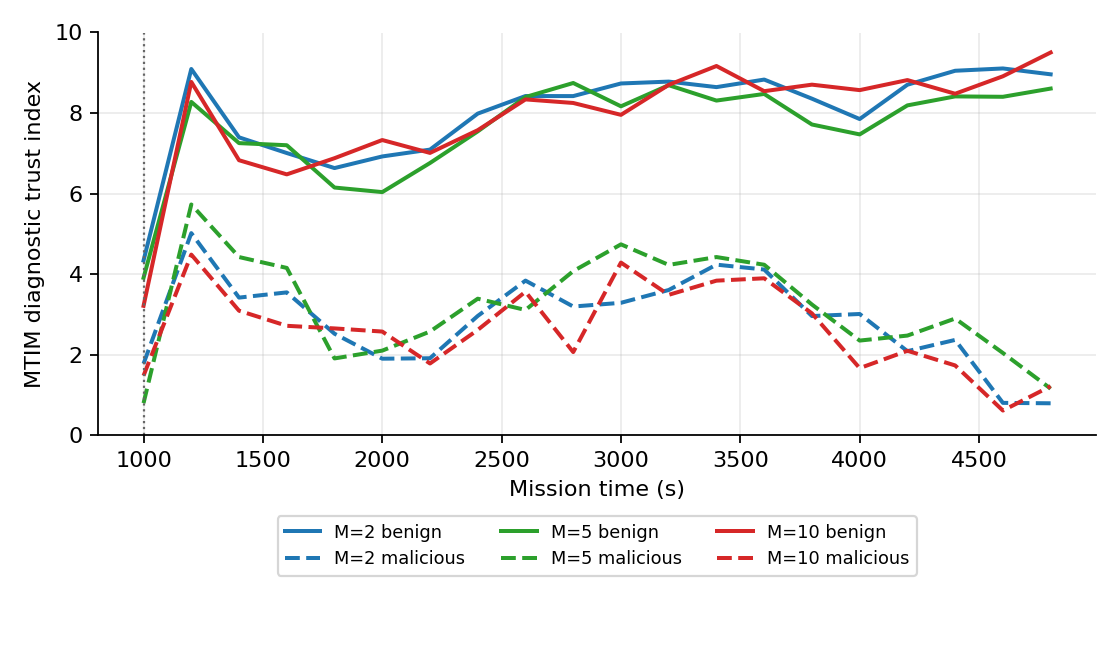
\includegraphics[width=0.72\textwidth]{trust_value_evolution.png}
\caption{Diagnostic trust index on generated streams for three seed conditions labeled by $M$. Since $M$ is not a policy feature, the curves do not identify a causal agent-count effect. Lower values indicate higher predicted risk.}
\label{fig:trust_value_evolution}
\end{figure}

\subsection{Comparative Performance Analysis}
\begin{figure}[!htbp]
\centering
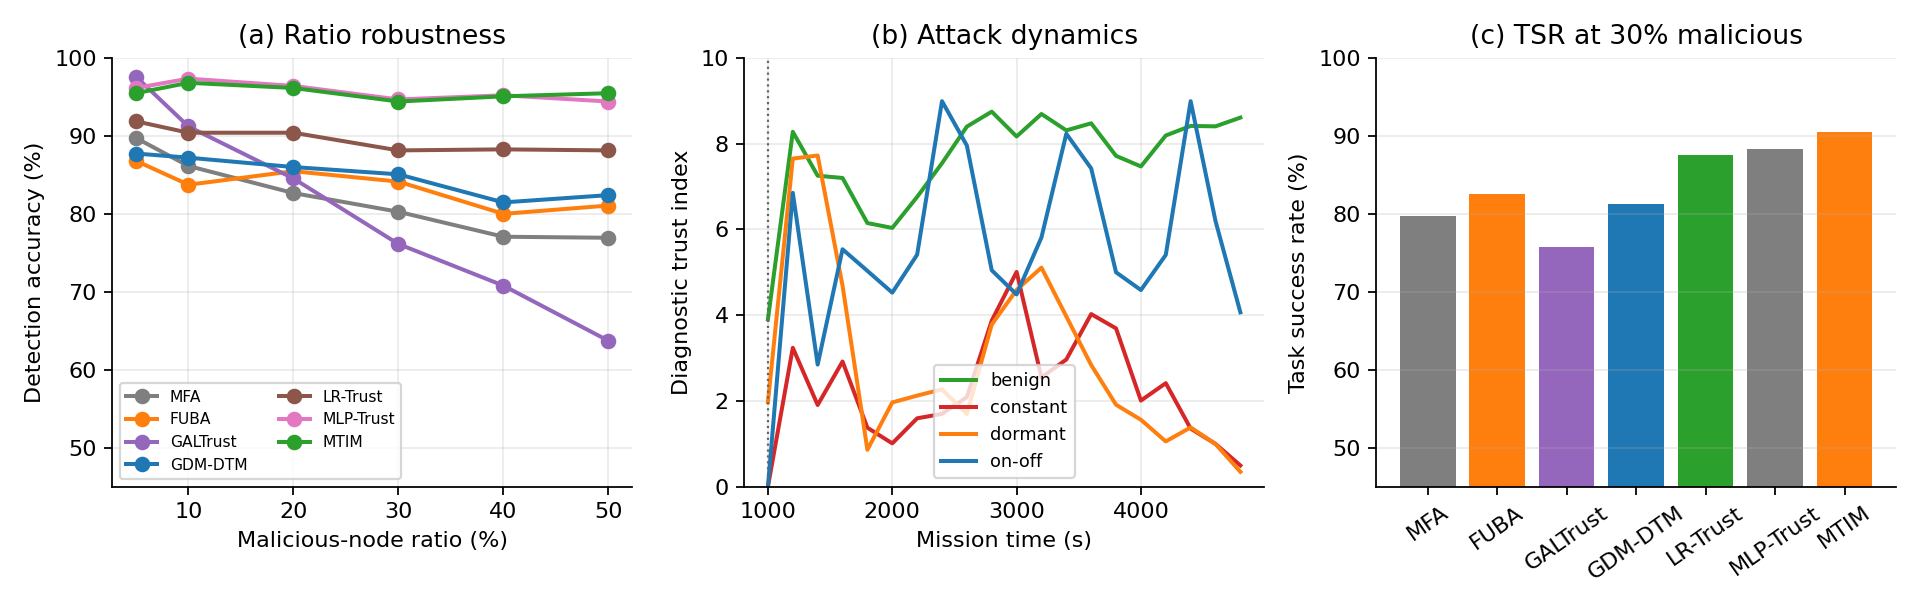
\includegraphics[width=\textwidth]{Fig5_energy_consumption.png}
\caption{Results from the generated trust-stream environment. (a) Detection accuracy across malicious-node ratios. (b) Diagnostic index for the generator's four behavior profiles. (c) Model-based task-success proxy at a 30\% malicious-node ratio.}
\label{fig:Fig5_energy_consumption}
\end{figure}

\textbf{Anti-manipulation under varying malicious ratios (Figure~\ref{fig:Fig5_energy_consumption}(a)).}
MTIM maintains high accuracy for malicious ratios of 20\% and above, with 94.4\% accuracy at 30\% and 95.5\% at 50\%. MLP-Trust is a strong detection competitor under the same features, confirming that the diagnostic feature set itself carries substantial discriminative information. GALTrust is highly accurate at 5--10\% malicious ratios but falls to 63.7\% at 50\%, indicating that the profile-distance adapter becomes unstable when the attack population substantially shifts the empirical trust distribution. MTIM does not show monotonic degradation across this generated ratio grid; this is favorable for the bounded setting but should be interpreted cautiously because stronger collusion and adaptive poisoning are not modeled.

\textbf{Trust dynamics under attack patterns (Figure~\ref{fig:Fig5_energy_consumption}(b)).}
Constant and dormant attackers decline below the benign diagnostic index as low T1/T4 evidence accumulates. Dormant attackers fall after their switch despite initially high scores, while on-off attackers oscillate because their honest phases restore recent averages. This behavior supports a conservative interpretation: MTIM identifies many on-off attackers as high risk, but their oscillatory trajectory remains the hardest case and drives the wide F-score variance in Table~\ref{tab:baseline_comparison}.

\textbf{Task success comparison (Figure~\ref{fig:Fig5_energy_consumption}(c)).}
MTIM has the highest simulated proxy (90.5\%), followed by MLP-Trust (88.3\%) and LR-Trust (87.6\%). This ordering is partly built into the allocation function, which applies MTIM-specific multipliers. It is not evidence that the auxiliary incentive head learned a better policy.\par

\textbf{Stress cases not claimed.}
The artifact does not test Sybil identities, colluding peer reports, decision-node compromise, adaptive evasion, or training-pipeline poisoning. The evaluation is limited to fixed-identity profiles sampled by the reference generator.

\paragraph{ns-3 trace-driven sanity check.}
To connect the trust-stream interface to packet/mobility observations, we converted the bundled 500~s ns-3-derived trace into T1--T5 streams and evaluated all methods on the converted trace. This is a single seed-1000 trace with 15 UAVs, 49 update steps, 10 benign nodes, three constant attackers, and two on-off attackers; it is not a multi-seed packet-level validation. Table~\ref{tab:ns3_trace_validation} shows that MTIM correctly preserves all benign nodes but detects only two of five malicious nodes on this short trace. In this trace-only setting, MFA, FUBA, and GDM-DTM detect three malicious nodes. Therefore, the ns-3 trace path should be interpreted as an interface-validation sanity check and as evidence that packet-level validation can expose harder short-horizon behavior than the main trust-stream simulator.

\begin{table}[!htbp]
  \centering
  \caption{Trace-driven validation on the bundled 500~s ns-3-derived trust stream (single seed, 15 UAVs, 49 update steps).}
  \label{tab:ns3_trace_validation}
  \footnotesize
  \setlength{\tabcolsep}{6pt}
  \renewcommand{\arraystretch}{1.12}
  \begin{tabular}{l c c c c c c}
    \toprule
    Method & Accuracy & Precision & Recall & F-score & TP/TN/FP/FN & Mean score (B/M) \\
    \midrule
    MFA & 86.7\% & 100.0\% & 60.0\% & 75.0\% & 3/10/0/2 & 0.900/0.619 \\
    FUBA & 86.7\% & 100.0\% & 60.0\% & 75.0\% & 3/10/0/2 & 0.939/0.574 \\
    GALTrust & 66.7\% & 50.0\% & 60.0\% & 54.5\% & 3/7/3/2 & 0.718/0.428 \\
    GDM-DTM & 86.7\% & 100.0\% & 60.0\% & 75.0\% & 3/10/0/2 & 0.938/0.586 \\
    LR-Trust & 80.0\% & 100.0\% & 40.0\% & 57.1\% & 2/10/0/3 & 1.000/0.600 \\
    MLP-Trust & 80.0\% & 100.0\% & 40.0\% & 57.1\% & 2/10/0/3 & 1.000/0.584 \\
    MTIM (ours) & 80.0\% & 100.0\% & 40.0\% & 57.1\% & 2/10/0/3 & 1.000/0.482 \\
    \bottomrule
  \end{tabular}
\end{table}
\subsection{Ablation Study}
\label{sec:ablation}
Table~\ref{tab:ablation} reports code-level variants. These are not clean single-component ablations: several rows replace the trained model with a hand-coded scoring rule, add noise, or subtract a fixed 0.09 from the task-success proxy. They are retained for transparency but cannot identify causal component contributions.

\begin{table}[!htbp]
  \centering
  \caption{Ablation study of MTIM components (30\% malicious-node ratio, 15 UAVs). All values are mean $\pm$ std over 50 trials.}
  \label{tab:ablation}
  \footnotesize
  \setlength{\tabcolsep}{6pt}
  \renewcommand{\arraystretch}{1.15}
  \resizebox{\textwidth}{!}{%
  \begin{tabular}{l c c c}
    \toprule
    \textbf{Code-level variant} & \textbf{Accuracy} & \textbf{F-score} & \textbf{TSR proxy} \\
    \midrule
    MTIM (full) & 94.4\% $\pm$ 5.6\% & 91.8\% $\pm$ 7.9\% & 90.5\% $\pm$ 3.7\% \\
    \midrule
    w/o Cross-factor Checking & 92.9\% $\pm$ 5.9\% & 89.5\% $\pm$ 8.6\% & 89.5\% $\pm$ 4.2\% \\
    w/o Bayesian Aggregation & 84.1\% $\pm$ 6.1\% & 67.7\% $\pm$ 16.2\% & 81.9\% $\pm$ 4.1\% \\
    w/o Temporal Decay & 79.5\% $\pm$ 6.1\% & 52.8\% $\pm$ 20.5\% & 80.0\% $\pm$ 3.8\% \\
    w/o Adaptive Policy & 82.3\% $\pm$ 7.0\% & 64.2\% $\pm$ 18.2\% & 80.9\% $\pm$ 4.5\% \\
    w/o Incentive Mechanism & 94.3\% $\pm$ 5.7\% & 91.7\% $\pm$ 8.0\% & 81.4\% $\pm$ 3.7\% \\
    \midrule
    T1 Only & 80.8\% $\pm$ 11.5\% & 74.9\% $\pm$ 14.2\% & 82.6\% $\pm$ 4.5\% \\
    T2 Only & 63.7\% $\pm$ 11.7\% & 53.3\% $\pm$ 13.8\% & 76.2\% $\pm$ 5.1\% \\
    T3 Only & 57.6\% $\pm$ 12.2\% & 56.0\% $\pm$ 9.8\% & 75.9\% $\pm$ 6.1\% \\
    T4 Only & 82.3\% $\pm$ 10.1\% & 76.5\% $\pm$ 12.9\% & 83.2\% $\pm$ 4.3\% \\
    T5 Only$^{\flat}$ & 84.0\% $\pm$ 9.7\% & 79.2\% $\pm$ 13.1\% & 82.6\% $\pm$ 3.9\% \\
    \bottomrule
  \end{tabular}}
  \vspace{2pt}
  \raggedright\scriptsize
  $^{\flat}$ T5-only applies exponential smoothing to T1--T4 without a learned model. It is one hand-coded temporal baseline, not an upper bound on temporal smoothing.
\end{table}

\paragraph{Analysis of Table~\ref{tab:ablation}.}
Only the cross-factor row resembles a feature ablation, and it also adds Gaussian noise. The ``Bayesian aggregation,'' ``temporal decay,'' and ``adaptive policy'' rows are alternative hand-coded classifiers rather than the full model with one component removed. The ``without incentive'' row perturbs risk and deducts 0.09 from TSR by construction. Consequently, the table is diagnostic of code paths, not evidence that any named architectural component causes the reported change.

\textbf{Single-branch baselines (T1--T5 only).}
Single-branch variants show that T4-only (82.3\%) and T5-only (84.0\%) are strong but insufficient; both trail MTIM by at least 10.4~pp in accuracy and by more than 7~pp in TSR. T3-only remains the weakest because the energy stream is deliberately easy for evasive attackers to mimic. These results support multi-factor temporal fusion, while also revealing that the current model places most discriminative power in behavior/task-history channels.

\subsection{Scalability and Sensitivity Analysis}
\label{sec:scalability}
We also vary the number of generated nodes from 5 to 50. Accuracy is empirical; time and communication values are formula outputs rather than measurements.

\begin{table}[!htbp]
  \centering
  \caption{Generated-node-count sensitivity under a 30\% malicious-node ratio. Time and communication columns are formula outputs, not measurements.}
  \label{tab:scalability}
  \footnotesize
  \setlength{\tabcolsep}{6pt}
  \renewcommand{\arraystretch}{1.12}
  \begin{tabular}{c c c c c}
    \toprule
    UAV count $N$ & Seed parameter $M$ & Accuracy (\%) & Time model (ms) & Cost model (KB/UAV) \\
    \midrule
    5  & 2  & $97.2 \pm 7.0$ & $36.5 \pm 3.0$ & $27.1 \pm 1.9$ \\
    15 & 5  & $94.4 \pm 5.6$ & $58.3 \pm 4.3$ & $34.0 \pm 1.8$ \\
    30 & 10 & $93.5 \pm 3.8$ & $95.1 \pm 4.2$ & $44.9 \pm 1.9$ \\
    50 & 17 & $95.2 \pm 2.9$ & $152.0 \pm 3.8$ & $59.8 \pm 1.7$ \\
    \bottomrule
  \end{tabular}
\end{table}

Detection accuracy stays above 93\% on the generated size grid. The apparent growth in time and communication is predetermined by \texttt{resource\_metrics}; no scaling law can be inferred from those columns.

Sensitivity analysis is limited to the fitted architecture, fixed threshold, and one trust-stream generator. Loss weights, temporal windows, threshold calibration, and distribution shift have not been studied systematically.

\subsection{Trust Factor Correlation Analysis}
To verify that the five trust dimensions capture complementary rather than redundant information, we computed the pairwise Pearson correlation coefficients among $T_i^{(1)}$ through $T_i^{(5)}$ across all UAVs and time steps in the 50-trial simulation set. The correlation matrix (averaged over trials) is:

\begin{table}[!htbp]
  \centering
  \caption{Pairwise Pearson correlations among the five trust dimensions (mean $\pm$ std over 50 trials).}
  \label{tab:correlation}
  \footnotesize
  \resizebox{\textwidth}{!}{%
  \begin{tabular}{l c c c c c}
    \toprule
    & T1 (Behavior) & T2 (Comm.) & T3 (Energy) & T4 (Task) & T5 (History) \\
    \midrule
    T1 & 1.00 & $0.28 \pm 0.10$ & $0.11 \pm 0.08$ & $0.41 \pm 0.10$ & $0.64 \pm 0.08$ \\
    T2 & -- & 1.00 & $0.13 \pm 0.09$ & $0.27 \pm 0.10$ & $0.51 \pm 0.07$ \\
    T3 & -- & -- & 1.00 & $0.11 \pm 0.09$ & $0.34 \pm 0.09$ \\
    T4 & -- & -- & -- & 1.00 & $0.65 \pm 0.09$ \\
    T5 & -- & -- & -- & -- & 1.00 \\
    \bottomrule
  \end{tabular}}
\end{table}

The strongest correlations involve the historical trust dimension T5, especially with T4 ($0.65 \pm 0.09$) and T1 ($0.64 \pm 0.08$), which is expected because T5 is an exponential history of recent trust evidence. Among the instantaneous dimensions T1--T4, all correlations remain at or below 0.41. Thus, T5 should be interpreted as a temporal memory channel rather than an independent sensor, while the instantaneous factors retain enough diversity to justify multi-factor fusion.

\section{Conclusions}
\label{sec:conclusions}

This study provides a reproducible trust-stream benchmark and a supervised multi-head risk model for UAV task allocation. On held-out seeds from the same generator, the model reaches 94.4\% accuracy and a 91.8\% F-score. A same-feature MLP reaches 94.7\% and 92.1\%; the paired differences are not significant. The principal empirical result is therefore that the chosen temporal summaries are informative for this generator, not that the proposed architecture is a better detector.

The 90.5\% task-success value is a simulator-specific proxy. Since the allocation code applies MTIM-specific multipliers and does not use the learned incentive head, the 2.2~pp difference from MLP-Trust cannot support a causal claim about incentive learning. Likewise, the reported communication and latency values are generated rather than measured, and the code-level ablations do not isolate named architectural components. The short ns-3-derived check is the most useful warning: MTIM detects only two of five malicious nodes and does not outperform the simpler adapters.

The repository is nevertheless useful as an auditable starting point. A defensible next study should replace the synthetic allocation rules with a common policy for all detectors, measure actual runtime and messages, implement genuine agent-local observations and aggregation, and evaluate on multi-seed packet traces with attack parameters held out from training. Reinforcement-learning claims would additionally require environment interaction, reward-defined returns, and comparison with supervised and non-learning policies. Until those experiments are available, MTIM should be described as a supervised trust-stream proof of concept rather than a validated MARL or zero-trust deployment.

%%%%%%%%%%%%%
\vspace{6pt} 

%%%%%%%%%%%%%
% optional
%\supplementary{The following supporting information can be downloaded at:  \linksupplementary{s1}, Figure S1: title; Table S1: title; Video S1: title.}

% Only for journal Methods and Protocols:
% If you wish to submit a video article, please do so with any other supplementary material.
% \supplementary{The following supporting information can be downloaded at: \linksupplementary{s1}, Figure S1: title; Table S1: title; Video S1: title. A supporting video article is available at doi: link.}

% Only used for preprtints:
% \supplementary{The following supporting information can be downloaded at the website of this paper posted on \href{https://www.preprints.org/}{Preprints.org}.}

% Only for journal Hardware:
% If you wish to submit a video article, please do so with any other supplementary material.
% \supplementary{The following supporting information can be downloaded at: \linksupplementary{s1}, Figure S1: title; Table S1: title; Video S1: title.\vspace{6pt}\\
%\begin{tabularx}{\textwidth}{lll}
%\toprule
%\textbf{Name} & \textbf{Type} & \textbf{Description} \\
%\midrule
%S1 & Python script (.py) & Script of python source code used in XX \\
%S2 & Text (.txt) & Script of modelling code used to make Figure X \\
%S3 & Text (.txt) & Raw data from experiment X \\
%S4 & Video (.mp4) & Video demonstrating the hardware in use \\
%... & ... & ... \\
%\bottomrule
%\\end{tabularx}
%}

%%%%%%%%%%%%%
\authorcontributions{All authors contributed to the conceptualization, methodology, analysis, and manuscript preparation. Author roles will be specified in the camera-ready version.}

\funding{This research received no external funding.}

\institutionalreview{Not applicable.}

\informedconsent{Not applicable.}

\dataavailability{The replication package is included under \texttt{artifacts/}. It provides the code, configurations, trained models, evaluation outputs, statistical summaries, generated figures, baseline reimplementations, and packet-trace conversion materials needed to reproduce the trust-layer results reported in this manuscript. The included packet-trace validation is a single short sanity check rather than a multi-seed packet-level validation dataset.}

\conflictsofinterest{The authors declare no conflict of interest.}

\reftitle{References}

% Please provide the correct journal abbreviation (e.g. according to the "List of Title Word Abbreviations" http://www.issn.org/services/online-services/access-to-the-ltwa/).
% Citations and References in Supplementary files are permitted provided that they also appear in the reference list here.

\begin{thebibliography}{999}
\bibitem{kundu2024survey}
Kundu, J.; Alam, S.; Das, J.C.; Dey, A.; Bari, S. Trust-Based Flying Ad Hoc Network: A Survey. {\em IEEE Access} {\bf 2024}, {\em 12}, 99258--99281.

\bibitem{noor2020fanet}
Noor, F.; Khan, M.A.; Al-Zahrani, A.; Ullah, I.; Al-Dhlan, K.A. A Review on Communications Perspective of Flying Ad-Hoc Networks: Key Enabling Wireless Technologies, Applications, Challenges and Open Research Topics. {\em Drones} {\bf 2020}, {\em 4}, 65.

\bibitem{brik2020fluav}
Brik, B.; Ksentini, A.; Bouaziz, M. Federated Learning for UAVs-Enabled Wireless Networks: Use Cases, Challenges, and Open Problems. {\em IEEE Netw.} {\bf 2020}, {\em 34}, 144--150.

\bibitem{nguyen2021fliotsurvey}
Nguyen, D.C.; Ding, M.; Pathirana, P.N.; Seneviratne, A.; Li, J.; Poor, H.V. Federated Learning for Internet of Things: A Comprehensive Survey. {\em IEEE Commun. Surv. Tutor.} {\bf 2021}, {\em 23}, 1622--1658.

\bibitem{qu2021dflun}
Qu, Y.; Dai, H.; Zhuang, Y.; Chen, J.; Dong, C.; Wu, F.; Guo, S. Decentralized Federated Learning for UAV Networks: Architecture, Challenges, and Opportunities. {\em IEEE Netw.} {\bf 2021}, {\em 35}, 156--162.

\bibitem{zuo2023blockchain}
Zuo, J.; Cao, R.; Qi, J.; Gao, P.; Wang, Z.; Li, J.; Zhang, L.; Lu, Y. A Hierarchical Blockchain-Based Trust Measurement Method for Drone Cluster Nodes. {\em Drones} {\bf 2023}, {\em 7}, 627.

\bibitem{ge2021uavpro}
Ge, C.; Zhou, L.; Hancke, G.P.; Su, C. A Provenance-Aware Distributed Trust Model for Resilient Unmanned Aerial Vehicle Networks. {\em IEEE Internet Things J.} {\bf 2021}, {\em 8}, 12481--12489.

\bibitem{benfriha2024fuba}
Benfriha, S.; Labraoui, N.; Bensaid, R.; Bany Salameh, H.; Saidi, H. FUBA: A Fuzzy-Based Unmanned Aerial Vehicle Behaviour Analytics for Trust Management in Flying Ad-Hoc Networks. {\em IET Networks} {\bf 2024}, {\em 13}, 208--220.

\bibitem{li2025multigranularity}
Li, H.; Li, X.; Dunkin, F.; Zhang, Z.; Lu, X. Adaptive Multi-Granularity Trust Management Scheme for UAV Visual Sensor Security under Adversarial Attacks. {\em Comput. Secur.} {\bf 2025}, {\em 148}, 104108.

\bibitem{akram2024galtrust}
Akram, J.; Anaissi, A.; Rathore, R.S.; Jhaveri, R.H.; Akram, A. GALTrust: Generative Adversarial Learning-Based Framework for Trust Management in Spatial Crowdsourcing Drone Services. {\em IEEE Trans. Consum. Electron.} {\bf 2024}, {\em 70}, 6196--6207.

\bibitem{ceviz2025flids}
Ceviz, O.; Sadioglu, P.; Sen, S.; Vassilakis, V.G. A Novel Federated Learning-Based IDS for Enhancing UAVs Privacy and Security. {\em Internet Things} {\bf 2025}, {\em 31}, 101592.

\bibitem{lu2024swarmfl}
Lu, Y.; Yang, T.; Zhao, C.; Chen, W.; Liu, Y.; Zeng, R. A Swarm Anomaly Detection Model for IoT UAVs Based on a Multi-Modal Denoising Autoencoder and Federated Learning. {\em Comput. Ind. Eng.} {\bf 2024}, {\em 196}, 110454.

\bibitem{gad2024somkd}
Gad, G.; Farrag, A.; Aboulfotouh, A.; Bedda, K.; Fadlullah, Z.M.; Fouda, M.M. Joint Self-Organizing Maps and Knowledge-Distillation-Based Communication-Efficient Federated Learning for Resource-Constrained UAV-IoT Systems. {\em IEEE Internet Things J.} {\bf 2024}, {\em 11}, 34270--34282.

\bibitem{wang2026wolf}
Wang, X.; Yuan, Q.; Liu, C.; Wang, P.; Tao, J.; Li, L.; Wang, X.; Wang, Y. Who Is the Wolf in Sheep's Clothing? A Context-Aware Trust Evaluation Model for Malicious UAV Detection during Authentication. {\em Comput. Netw.} {\bf 2026}, {\em 279}, 112145.

\bibitem{rose2020zero}
Rose, S.; Borchert, O.; Mitchell, S.; Connelly, S. Zero Trust Architecture. {\em NIST Spec. Publ.} {\bf 2020}, {\em 800-207}, 1--59.

\bibitem{ekechi2025survey}
Ekechi, C.C.; Elfouly, T.; Alouani, A.; Khattab, T. A Survey on UAV Control with Multi-Agent Reinforcement Learning. {\em Drones} {\bf 2025}, {\em 9}, 484.

\bibitem{akram2024tmiodt}
Akram, J.; Anaissi, A.; Rathore, R.S.; Jhaveri, R.H.; Akram, A. Digital Twin-Driven Trust Management in Open RAN-Based Spatial Crowdsourcing Drone Services. {\em IEEE Trans. Green Commun. Netw.} {\bf 2024}, {\em 8}, 1061--1075.

\bibitem{abubaker2022blockchained}
Abubaker, Z.; Javaid, N.; Almogren, A.; Akbar, M.; Zuair, M.; Ben-Othman, J. Blockchained Service Provisioning and Malicious Node Detection via Federated Learning in Scalable Internet of Sensor Things Networks. {\em IEEE Trans. Netw. Serv. Manag.} {\bf 2023}, {\em 20}, 1847--1865.

\bibitem{akram2023chained}
Akram, J.; Umair, M.; Jhaveri, R.H.; Riaz, M.; Chi, H.R.; Malebary, S. Chained-Drones: Blockchain-Based Privacy-Preserving Framework for Secure and Intelligent Service Provisioning in Internet of Drone Things. {\em Comput. Electr. Eng.} {\bf 2023}, {\em 110}, 108772.

\bibitem{zheng2024tinyfl}
Zheng, J.; Xu, J.; Du, H.; Niyato, D.; Kang, J.; Nie, J.; Wang, Z. Trust Management of Tiny Federated Learning in Internet of Unmanned Aerial Vehicles. {\em IEEE Internet Things J.} {\bf 2024}, {\em 11}, 21046--21060.

\bibitem{tong2024hierarchicalfl}
Tong, Z.; Wang, J.; Hou, X.; Chen, J.; Jiao, Z.; Liu, J. Blockchain-Based Trustworthy and Efficient Hierarchical Federated Learning for UAV-Enabled IoT Networks. {\em IEEE Internet Things J.} {\bf 2024}, {\em 11}, 15504--15522.

\bibitem{trustgame_qfl_uav}
Xu, Q.; Li, R.; Qi, Y.; Su, Z.; Fang, D. Trust-Enhanced Game Incentive for Secure Quantum Federated Learning in UAV-Assisted Wireless Networks. {\em IEEE J. Sel. Areas Commun.} {\bf 2025}, {\em 43}, 2841--2856.

\bibitem{hu2025gdm}
Hu, Y.; Gan, Y.; Wu, H.; Wang, C.; Ma, M.; Xiong, C. GDM-DTM: A Group Decision-Making-Enabled Dynamic Trust Management Method for Malicious Node Detection in Low-Altitude UAV Networks. {\em Sensors} {\bf 2025}, {\em 25}, 3982.

\bibitem{wang2025continuous}
Wang, X.; Yuan, Q.; Wang, Y.; Teng, J.; Tao, J.; Shen, M. Zero Trust-Driven Collaborative Intrusion Detection in Internet of Things: A Continuous Trust Assessment Approach. {\em IEEE Internet Comput.} {\bf 2025}, {\em 29}, 37--47.

\bibitem{ridhawi2023zerotrust6g}
Al Ridhawi, I.; Aloqaily, M. Zero-Trust UAV-Enabled and DT-Supported 6G Networks. {\em IEEE Internet Comput.} {\bf 2023}, {\em 27}, 59--67.

\bibitem{wang2020trajectory}
Wang, L.; Wang, K.; Pan, C.; Xu, W.; Aslam, N.; Hanzo, L. Multi-Agent Deep Reinforcement Learning Based Trajectory Planning for Multi-UAV Assisted Mobile Edge Computing. {\em IEEE Trans. Cogn. Commun. Netw.} {\bf 2021}, {\em 7}, 73--84.

\bibitem{nie2021resource}
Nie, Y.; Zhao, J.; Gao, F.; Yu, F.R. Semi-Distributed Resource Management in UAV-Aided MEC Systems: A Multi-Agent Federated Reinforcement Learning Approach. {\em IEEE Trans. Veh. Technol.} {\bf 2021}, {\em 70}, 13162--13173.

\bibitem{alam2024joint}
Alam, M.M.; Moh, S. Joint Optimization of Trajectory Control, Task Offloading, and Resource Allocation in Air-Ground Integrated Networks. {\em IEEE Internet Things J.} {\bf 2024}, {\em 11}, 24273--24288.

\bibitem{yang2021ppfluav}
Yang, H.; Zhao, J.; Xiong, Z.; Lam, K.-Y.; Sun, S.; Xiao, L. Privacy-Preserving Federated Learning for UAV-Enabled Networks: Learning-Based Joint Scheduling and Resource Management. {\em IEEE J. Sel. Areas Commun.} {\bf 2021}, {\em 39}, 3144--3159.

\bibitem{lim2021contractfl}
Lim, W.Y.B.; Huang, J.; Xiong, Z.; Kang, J.; Niyato, D.; Hua, X.-S.; Leung, C.; Miao, C. Towards Federated Learning in UAV-Enabled Internet of Vehicles: A Multi-Dimensional Contract-Matching Approach. {\em IEEE Trans. Intell. Transp. Syst.} {\bf 2021}, {\em 22}, 5140--5154.

\bibitem{wang2023hnpfl}
Wang, S.; Hosseinalipour, S.; Gorlatova, M.; Brinton, C.G.; Chiang, M. UAV-Assisted Online Machine Learning Over Multi-Tiered Networks: A Hierarchical Nested Personalized Federated Learning Approach. {\em IEEE Internet Things J.} {\bf 2024}, {\em 11}, 20899--20911.

\bibitem{qureshi2024asynfl}
Qureshi, K.I.; Wang, L.; Xiong, X.; Lodhi, M.A. Asynchronous Federated Learning for Resource Allocation in Software-Defined Internet of UAVs. {\em IEEE Internet Things J.} {\bf 2024}, {\em 11}, 15523--15538.

\bibitem{jing2023agifl}
Jing, Y.; Qu, Y.; Dong, C.; Ren, W.; Shen, Y.; Wu, Q.; Guo, S. Exploiting UAV for Air-Ground Integrated Federated Learning: A Joint UAV Location and Resource Optimization Approach. {\em IEEE Trans. Green Commun. Netw.} {\bf 2023}, {\em 7}, 1420--1433.

\bibitem{fu2025energyfl}
Fu, Z.; Liu, J.; Mao, Y.; Qu, L.; Xie, L.F.; Wang, X. Energy-Efficient UAV-Assisted Federated Learning: Trajectory Optimization, Device Scheduling, and Resource Management. {\em IEEE Trans. Netw. Serv. Manag.} {\bf 2025}, {\em 22}, 974--988.

\bibitem{cao2025sagin}
Cao, X.; Nan, G.; Guo, H.; Mu, H.; Wang, L.; Lin, Y.; Zhou, Q.; Li, J.; Qin, B.; Cui, Q.; Tao, X.; Fang, H.; Du, H.; Quek, T.Q.S. Exploring LLM-Based Multi-Agent Situation Awareness for Zero-Trust Space-Air-Ground Integrated Network. {\em IEEE J. Sel. Areas Commun.} {\bf 2025}, {\em 43}, 2230--2247.

\bibitem{bertsekas1996reinforcement}
Bertsekas, D.P.; Tsitsiklis, J.N. {\em Neuro-Dynamic Programming}; Athena Scientific: Nashua, NH, USA, 1996.

\bibitem{oliehoek2008optimal}
Oliehoek, F.A.; Spaan, M.T.; Vlassis, N. Optimal and Approximate Solutions to Decentralized POMDPs. In {\em Proceedings of the 17th International Conference on Automated Planning and Scheduling (ICAPS)}; AAAI Press: 2008; pp. 274--281.

\bibitem{riley2010ns3}
Riley, G.F.; Henderson, T.R. The ns-3 Network Simulator. In {\em Modeling and Tools for Network Simulation}; Wehrle, K.; G{\"u}nes, M.; Gross, J., Eds.; Springer: Berlin, Germany, 2010; pp. 15--34.

\bibitem{hausknecht2015drqn}
Hausknecht, M.; Stone, P. Deep Recurrent Q-Learning for Partially Observable MDPs. In {\em Proceedings of the AAAI Fall Symposium on Sequential Decision Making for Intelligent Agents}; AAAI Press: 2015; pp. 29--37.

\bibitem{hausknecht2016parameterized}
Hausknecht, M.; Stone, P. Deep Reinforcement Learning in Parameterized Action Space. In {\em Proceedings of the International Conference on Learning Representations (ICLR)}; 2016.

\bibitem{xiong2018pdqn}
Xiong, J.; Wang, Q.; Yang, Z.; Sun, P.; Han, L.; Zheng, Y.; Fu, H.; Zhang, T.; Liu, J.; Liu, H. Parametrized Deep Q-Networks Learning: Reinforcement Learning with Discrete-Continuous Hybrid Action Space. {\em arXiv} {\bf 2018}, arXiv:1810.06394.
\end{thebibliography}

\end{document}
